\chapter{Resultados} \label{resultado}

Nós inicialmente analisamos erro e discrepância nos 12.502 endereços de São Paulo. Abaixo estão os totais de geocodificações bem-sucedidas para cada API:

\begin{itemize}
    \item TomTom: 11.370 endereços;
    \item Google Maps: 9.389 endereços;
    \item Mapbox: 12.260 endereços;
    \item ORS: 12.295 endereços.
\end{itemize}

Então, conduzimos experimentos com o conjunto de dados de Belo Horizonte. Em relação ao número de endereços retornados, as APIs retornaram da base de 85.000:

\begin{itemize}
    \item TomTom: 84.981 endereços;
    \item Google: 84.941 endereços;
    \item Mapbox: 84.966 endereços; 
    \item ORS: 84.864 endereços.
\end{itemize}    

Falhas podem ocorrer em qualquer estágio de geocodificação, derivadas de informações incompletas ou ambíguas fornecidas para geocodificação ou dos algoritmos empregados (algoritmos de seleção e classificação de candidatos). Quando falhas ocorrem, a API retorna apenas uma mensagem de erro. Nas próximas seções, os resultados de erro e discrepância são cuidadosamente analisados.

\section{Erro, Taxa de Resposta e Taxa de Precisão}

A próxima etapa foi o calculo do erro para cada um dos pontos, sendo este expresso em quilômetros (Km).

Com o erro de cada um dos pontos, foram calculadas as métricas mencionadas anteriormente. Os resultados bem como suas interpretações são apresentados abaixo.

A Tabela \ref{tab:tabelaDeMetricasSP} apresenta os resultados calculados para as respostas recebidas da geocodificação da base de São Paulo. Em relação à taxa de resposta, ou seja, o número de endereços que foram geocodificados com sucesso, a Mapbox obteve o melhor resultado, seguida pela ORS, ambas com taxas de resposta superiores a 98\%. Google e TomTom tiveram taxas de resposta de 75\% e 90\%, respectivamente. Esses resultados são considerados satisfatórios e garantem uma boa quantidade de dados para as avaliações subsequentes.

\begin{table}[!ht]
    \centering
    \caption{Métricas de Erro para São Paulo}
    \label{tab:tabelaDeMetricasSP}
    \begin{adjustbox}{width=0.7\textwidth}
    \begin{tabular}{|c|c|c|c|}
    \hline
    API & Média (km) & Mediana (km) & Desvio Padrão \\
    \hline
    Mapbox & 15,3504 & 0,1675 & 83,9394 \\
    Google Maps & 2,0965 & 0,0555 & 22,0156 \\
    TomTom & 10,2074 & 0,0638 & 88,0844 \\
    ORS & 33,9474 & 1,2984 & 103,0119 \\
    \hline
    %\multicolumn{4}{c}{} \\ % Espaço em branco entre as tabelas
    \hline
    API & Média Aparada em 5\% (km) & Taxa de Resposta (\%) & Taxa de Precisão (\%) \\
    \hline
    Mapbox & 3,5009 & 98,0565 & 46,5968 \\
    Google Maps & 0,2327 & 75,0940 & 52,2675 \\
    TomTom & 0,4768 & 90,9382 & 60,3055 \\
    ORS & 16,4096 & 98,3364 & 28,6091 \\
    \hline
    \end{tabular}
    \end{adjustbox}
\end{table}

Outra métrica importante é a taxa de precisão. Endereços com erros menores que 150 metros (0,15 km) foram considerados precisos. A taxa de precisão foi baixa para a maioria das APIs. A API TomTom teve a maior taxa de precisão, com 60\% de acurácia.

O erro médio foi bastante elevado, variando de 2 km a 33 km. O desvio padrão também foi alto, indicando uma variação considerável no erro. No entanto, a mediana foi bastante baixa, alcançando resultados desejáveis em nossa pesquisa. A média aparada produziu resultados muito bons, indicando a presença de um número significativo de valores atípicos.

Da mesma forma, calculamos o erro para cada ponto geocodificado no banco de dados de Belo Horizonte e computamos as métricas mencionadas anteriormente. A Tabela \ref{tab:tabelaDeMetricasBH} exibe esses resultados.

\begin{table}[!ht]
    \centering
    \caption{Métricas de Erro para Belo Horizonte}
    \label{tab:tabelaDeMetricasBH}
    \begin{adjustbox}{width=0.7\textwidth}
    \begin{tabular}{|c|c|c|c|}
    \hline
    API & Média (km) & Mediana (km) & Desvio Padrão \\
    \hline
    Mapbox & 3,2857 & 0,0001 & 24,7587 \\
    Google Maps & 2,4924 & 0,0098 & 5,8465 \\
    TomTom & 11,2913 & 0,1147 & 56,6424 \\
    ORS & 6,4828 & 7,5702 & 5,5364 \\
    \hline
    %\multicolumn{4}{c}{} \\ % Espaço em branco entre as tabelas
    \hline
    API & Média Aparada em 5\% (km) & Taxa de Resposta (\%) & Taxa de Precisão (\%) \\
    \hline
    Mapbox & 1,0701 & 99,9600 & 76,8235 \\
    Google Maps & 1,6146 & 99,9306 & 73,6118 \\
    TomTom & 0,4768 & 99,9776 & 51,7988 \\
    ORS & 6,2940 & 99,8400 & 25,1835 \\
    \hline
    \end{tabular}
    \end{adjustbox}
\end{table}

Em relação à taxa de resposta, todas as APIs tiveram excelentes resultados, com mais de 99\% de resposta para o banco de dados fornecido. Este é um resultado significativo para a pesquisa, pois as conclusões são mais robustas devido à quantidade de dados analisados.

A taxa de precisão também mostrou resultados satisfatórios, com os melhores resultados vindos da Mapbox e Google Maps, com taxas superiores a 73\%. Este resultado é bastante satisfatório e está alinhado com os resultados obtidos em \cite{Clodoveu2011}. No entanto, TomTom e ORS apresentaram baixas taxas de precisão, sendo que ORS teve uma taxa extremamente baixa de 25\%. É importante observar que um resultado foi considerado preciso se o erro fosse menor ou igual a 150 metros.

O erro médio apresentou valores muito mais suaves do que os obtidos com o conjunto de dados de São Paulo, embora ainda estivessem elevados, variando de aproximadamente 2 a 11 quilômetros. Os valores medianos foram bastante baixos para a maioria das APIs, e o desvio padrão foi bastante alto. Esse resultado indica que também existem valores de erro muito altos nessa geocodificação. A API ORS apresentou resultados diferentes das outras APIs, com valores altos de média, mediana e desvio padrão, o que provavelmente explica a baixa taxa de precisão.

\section{Distribuição de Erro}

Com base nos resultados acima, realizamos uma análise da distribuição de erro para cada uma das GeoAPIs e bases. Para isso, utilizamos histogramas de erro individuais para cada API e os combinamos. As Figuras \ref{fig:hist-global-bh} e \ref{fig:hist-global-sp} mostram os histogramas para cada API e cada base utilizada. No entanto, devido à presença de alguns erros extremos, os histogramas gerais (que continham todo o conjunto de dados) não foram muito representativos, pois a maior parte do erro estava concentrada entre 0 km e 50 km, enquanto existiam erros bem maiores. Esse intervalo é considerado um erro muito grande, tornando desafiador tirar conclusões sólidas. Outra limitação dessa análise, é o fato de que cada API teve um máximo de erro diferente, prejudicando então a comparação entre APIs.

\begin{figure}[ht]
  \centering
  \begin{subfigure}[b]{0.45\textwidth}
    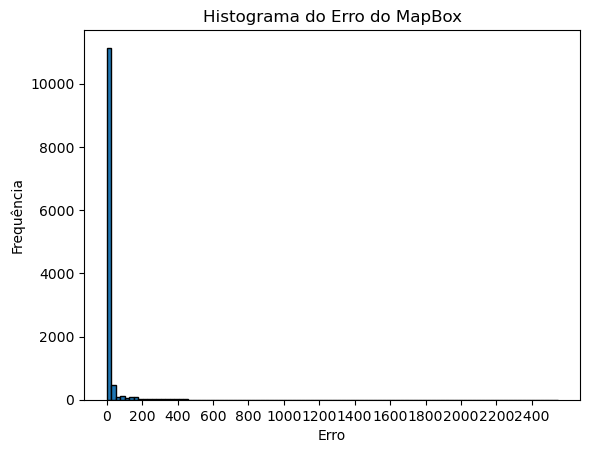
\includegraphics[width=\textwidth]{Figuras/histMapboxSP.png}
    \caption{Mapbox}
    \label{fig:histmapbox}
  \end{subfigure}
  \hfill
  \begin{subfigure}[b]{0.45\textwidth}
    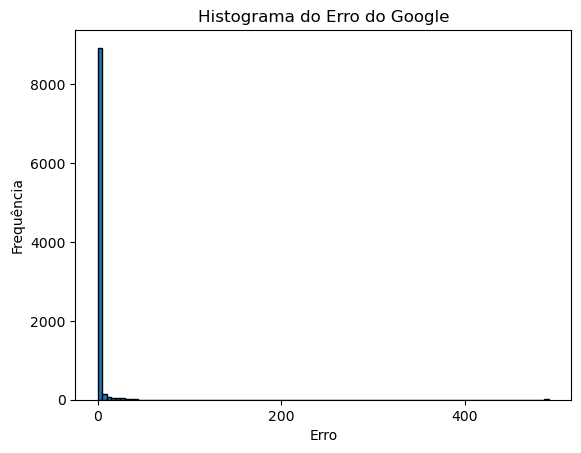
\includegraphics[width=\textwidth]{Figuras/histGoogleSP.png}
    \caption{Google}
    \label{fig:histgoogle}
  \end{subfigure}

  \begin{subfigure}[b]{0.45\textwidth}
    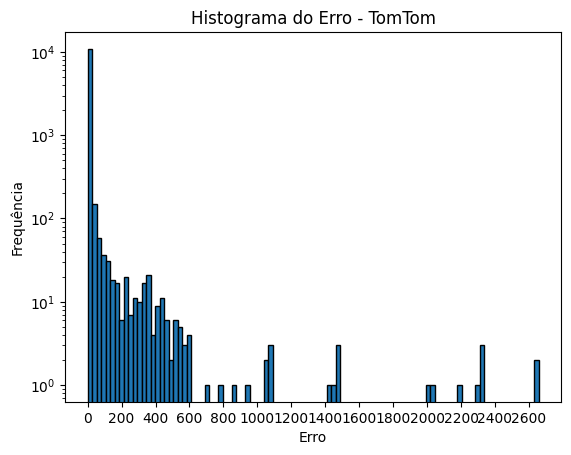
\includegraphics[width=\textwidth]{Figuras/histTomtomSP.png}
    \caption{TomTom}
    \label{fig:histtomtom}
  \end{subfigure}
  \hfill
  \begin{subfigure}[b]{0.45\textwidth}
    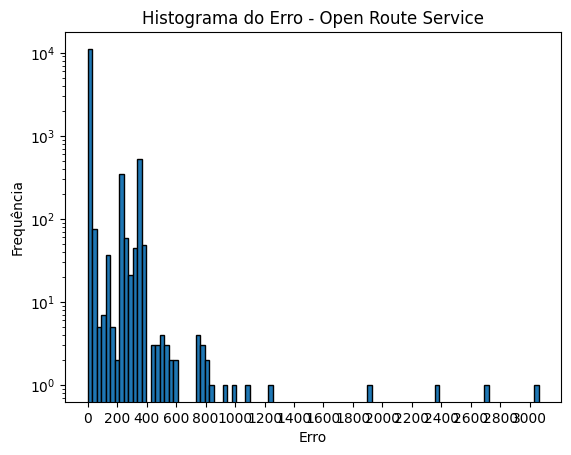
\includegraphics[width=\textwidth]{Figuras/histOrsSP.png}
    \caption{ORS}
    \label{fig:histors}
  \end{subfigure}
  
  \caption{Histogramas do erro das 4 APIs para o todos os dados de São Paulo}
  \label{fig:hist-global-sp}
\end{figure}


\begin{figure}[ht]
  \centering
  \begin{subfigure}[b]{0.45\textwidth}
    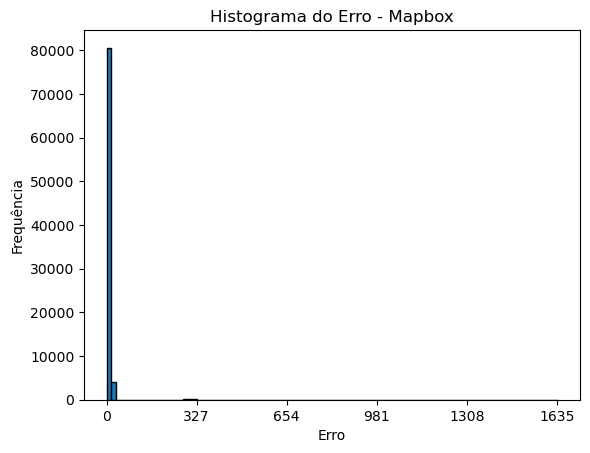
\includegraphics[width=\textwidth]{Figuras/histMapboxBH.png}
    \caption{Mapbox}
    \label{fig:histmapboxb}
  \end{subfigure}
  \hfill
  \begin{subfigure}[b]{0.45\textwidth}
    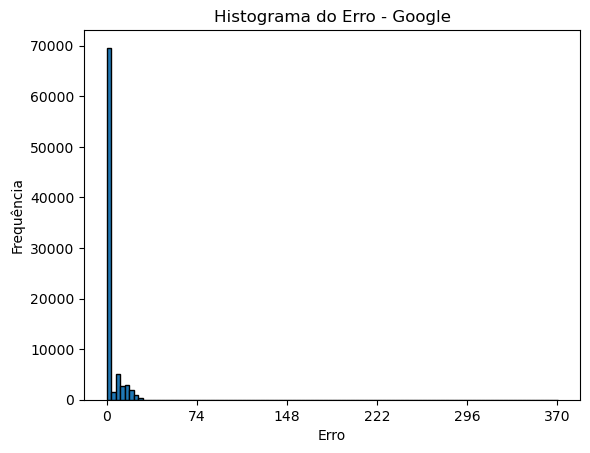
\includegraphics[width=\textwidth]{Figuras/histGoogleBH.png}
    \caption{Google}
    \label{fig:histgoogleB}
  \end{subfigure}

  \begin{subfigure}[b]{0.45\textwidth}
    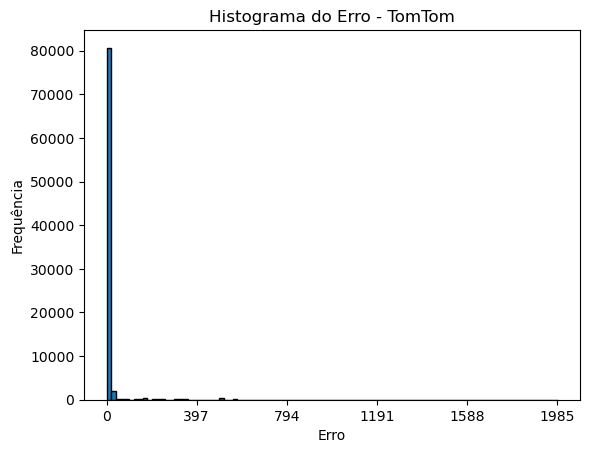
\includegraphics[width=\textwidth]{Figuras/histTomtomBH.png}
    \caption{TomTom}
    \label{fig:histtomtomB}
  \end{subfigure}
  \hfill
  \begin{subfigure}[b]{0.45\textwidth}
    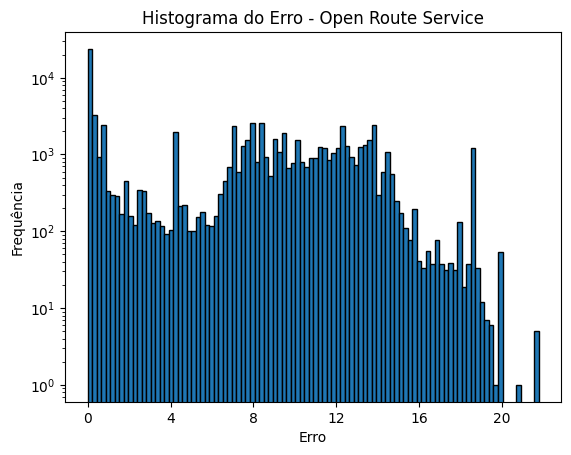
\includegraphics[width=\textwidth]{Figuras/histOrsBH.png}
    \caption{ORS}
    \label{fig:historsB}
  \end{subfigure}
  
  \caption{Histogramas do erro das 4 APIs para o todos os dados de Belo Horizonte}
  \label{fig:hist-global-bh}
\end{figure}

Portanto, decidimos cortar os dados, limitando o erro a 300 metros. Repetimos o processo, gerando um único histograma que representa a distribuição de erro para todas as APIs juntas, para cada uma das bases. 

A figura \ref{fig:histLimitadoSP} mostra o histograma resultante para os dados de São Paulo e a figura \ref{fig:histLimitadoBH} mostra o histograma para os dados de Belo Horizonte. 

Em relação aos dados de São Paulo as APIs tiveram resultados similares nessa faixa de valores do erro. Porém as APIs Google Maps e TomTom se destacaram ao conter uma curva mais estreira, ou seja, os valores para essas APIs estão mais concentrados em erro menor que 50 metros. 

Para os dados de Belo Horizonte, a API Mapbox teve melhores resultados com uma curva bem estreita. Seguida pela Google Maps, que apesar de ter uma curva bem estreita também, apresenta uma diferença significativa para a Mapbox. As outras APIs apresentam curvas mais largas e algo notável é a curva da ORS que está muito distribuída, tendo um aspecto parecido com uma reta em valores de erro superiores a 50 metros. Isso mostra que a ORS apresenta erro similar na maior parte da faixa, o que indica que ela não apresenta bons resultados nem quando há um corte nos dados.

\begin{figure}[h]
  \centering
  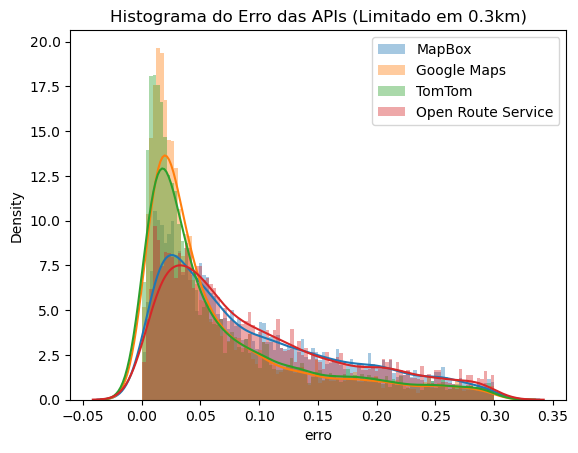
\includegraphics[width=0.7\textwidth]{Figuras/histLimitadoSP.png}
  \caption{Histograma comparativo de erro das APIs limitado em 300 metros para os dados de São Paulo}
  \label{fig:histLimitadoSP}
\end{figure}

\begin{figure}[h]
  \centering
  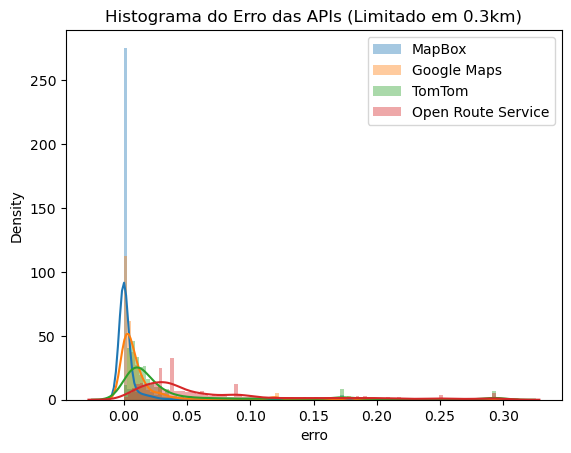
\includegraphics[width=0.7\textwidth]{Figuras/histLimitadoBH.png}
  \caption{Histograma comparativo de erro das APIs limitado em 300 metros para os dados de Belo Horizonte}
  \label{fig:histLimitadoBH}
\end{figure}

Em geral, embora os histogramas sejam uma ferramenta poderosa para analisar a distribuição de erros, neste caso, eles não se mostraram tão eficazes devido às limitações decorrentes da presença de valores excessivamente altos.

% \section{Distribuição Espacial do Erro}

% Além disso, realizamos uma análise adicional com o objetivo de verificar o comportamento do erro no espaço. Utilizamos gráficos de classificação hexagonal, empregando a função hexbin da biblioteca matplotlib, que desempenha um papel integral na construção do gráfico. Essa função automatiza o processo, dividindo o espaço em hexágonos de tamanhos uniformes e distribuídos de maneira equitativa. Em seguida, a função hexbin seleciona os pontos de dados contidos em cada hexágono e aplica uma função específica, que é definida como parâmetro da função hexbin. Essa função determina os cálculos realizados com base nos pontos, gerando um valor único. Esse valor é então atribuído ao hexágono correspondente no gráfico, e as cores são mapeadas de acordo com uma escala predefinida.

% Para gerar a representação do gráfico introduzimos o conceito de "falha". Quando o erro em um ponto específico é igual ou inferior a 150 metros, atribuímos o valor 0 à falha; caso contrário, designamos o valor 1. A função escolhida para calcular o valor de cada hexágono é a média da falha dos pontos, resultando em uma representação em porcentagem decimal da falha naquela região. Assim, quanto mais escura a cor do gráfico, maior é a falha observada. Para melhor vizualização, também adicionamos o limite da cidade como contorno do gráfico. As figuras \ref{fig:falhas-global-bh} e \ref{fig:falhas-global-sp} apresentam os gráficos de falhas de cada uma das APIs para os dados de Belo Horizonte e São Paulo respectivamente. 

% Para os dados de Belo Horizonte é possível notar que a API com gráfico mais claro, ou seja, menos falhas, é a Mapbox, seguido pela Google. Resultado que vai de encontro com os obtidos nas tabela de métricas \ref{tab:tabelaDeMetricasBH}. Outra informação relevante que é possível observar é que em todas as APIs existe uma concentração maior de falhas próximo aos limites da cidade, como esperado. Outro ponto importante é o gráfico da ORS. A maior parte do gráfico para essa API apresenta cores bem escuras, indicando muitas falhas em toda região da cidade para essa API. Mais especificamente nas regiões superior e inferior do gráfico o valor chega próximo do limite máximo, o que indica que naquela região houve aproximadamente 100\% de falha. Esse resultado, apesar de ruim, está de acordo com os análises sobre a ORS feitas anteriormente. 

% \begin{figure}[ht]
%   \centering
%   \begin{subfigure}[b]{0.45\textwidth}
%     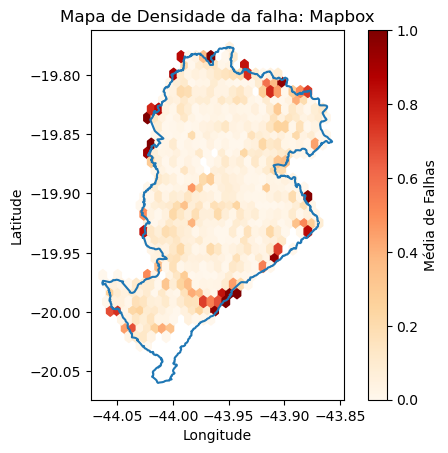
\includegraphics[width=\textwidth]{Figuras/falhasMapboxBH.png}
%     \caption{Mapbox}
%     \label{fig:falhasmapboxB}
%   \end{subfigure}
%   \hfill
%   \begin{subfigure}[b]{0.45\textwidth}
%     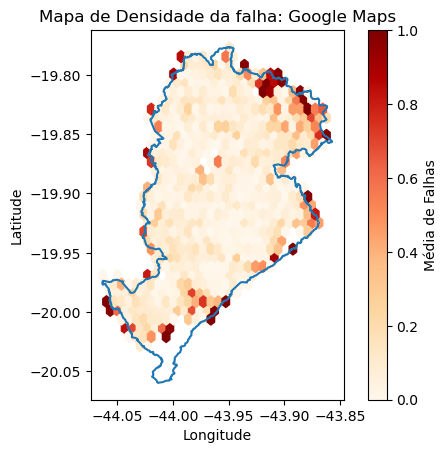
\includegraphics[width=\textwidth]{Figuras/falhasGoogleBH.png}
%     \caption{Google}
%     \label{fig:falhasgoogleB}
%   \end{subfigure}

%   \begin{subfigure}[b]{0.45\textwidth}
%     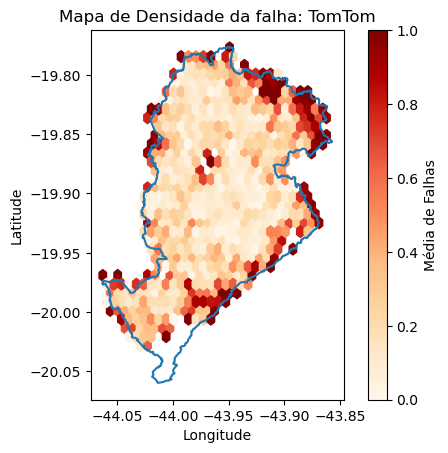
\includegraphics[width=\textwidth]{Figuras/falhasTomtomBH.png}
%     \caption{TomTom}
%     \label{fig:falhastomtomB}
%   \end{subfigure}
%   \hfill
%   \begin{subfigure}[b]{0.45\textwidth}
%     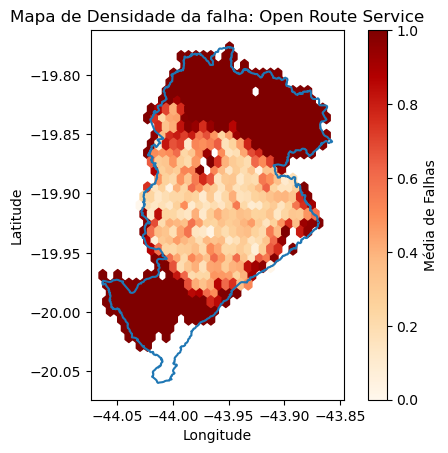
\includegraphics[width=\textwidth]{Figuras/falhasORSBH.png}
%     \caption{ORS}
%     \label{fig:falhasorsB}
%   \end{subfigure}
  
%   \caption{Gráficos de falhas de cada API para os dados de Belo Horizonte}
%   \label{fig:falhas-global-bh}
% \end{figure}

% Nos gráficos de São Paulo também foi adicionado o contorno da cidade. No entanto, os dados são referentes a região metropolitana, incluindo outras cidades da região. Para essa base é possível notar que as APIs Google Maps e TomTom tem melhores resultados, o que confirma os resultados obtidos na tabela \ref{tab:tabelaDeMetricasSP}. Outro resultado notável é que nos outros municípios o resultado piora em todas as APIs, atingindo valores de falha muito próximo de 1. Por fim, as APIs que foram piores foram Mapbox e ORS. A ORS foi claramente pior, repetindo os resultado de Belo Horizontes observados nos gráficos da figura \ref{fig:falhas-global-bh} e nas tabelas \ref{tab:tabelaDeMetricasBH} e \ref{tab:tabelaDeMetricasSP}.

% \begin{figure}[ht]
%   \centering
%   \begin{subfigure}[b]{0.45\textwidth}
%     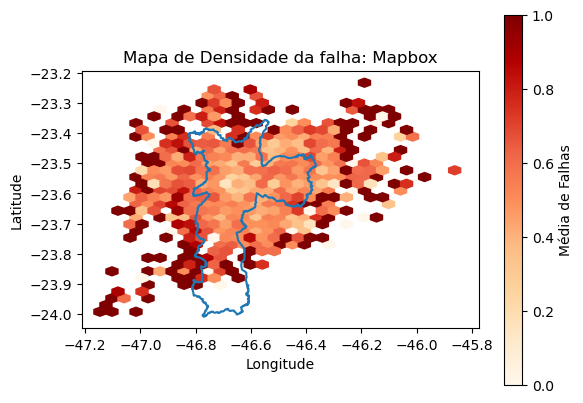
\includegraphics[width=\textwidth]{Figuras/falhasMapboxSP.png}
%     \caption{Mapbox}
%     \label{fig:falhasmapboxS}
%   \end{subfigure}
%   \hfill
%   \begin{subfigure}[b]{0.45\textwidth}
%     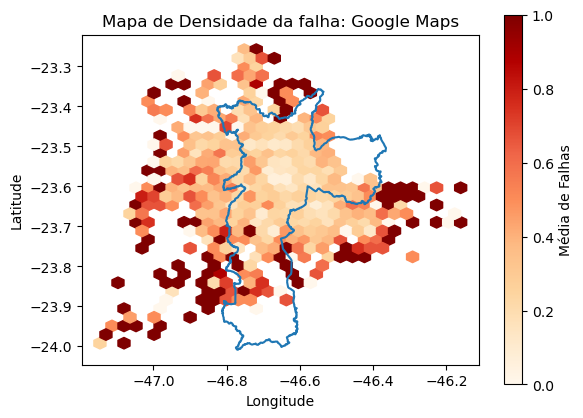
\includegraphics[width=\textwidth]{Figuras/falhasGoogleSP.png}
%     \caption{Google}
%     \label{fig:falhasgoogleS}
%   \end{subfigure}

%   \begin{subfigure}[b]{0.45\textwidth}
%     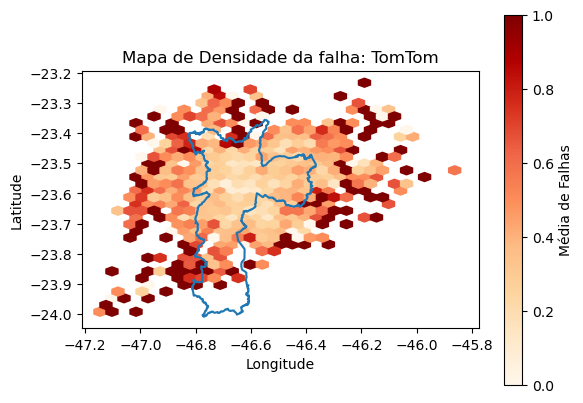
\includegraphics[width=\textwidth]{Figuras/falhasTomtomSP.png}
%     \caption{TomTom}
%     \label{fig:falhastomtomS}
%   \end{subfigure}
%   \hfill
%   \begin{subfigure}[b]{0.45\textwidth}
%     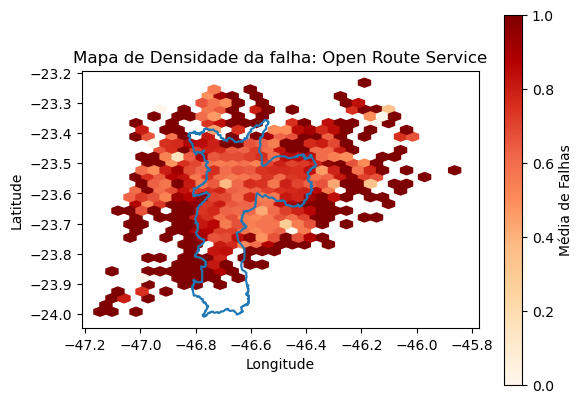
\includegraphics[width=\textwidth]{Figuras/falhasORSSP.png}
%     \caption{ORS}
%     \label{fig:falhasorsS}
%   \end{subfigure}
  
%   \caption{Gráficos de falhas de cada API para os dados de Belo São Paulo}
%   \label{fig:falhas-global-sp}
% \end{figure}

% \section{Relações entre erro e discrepância}

% Por fim, foi realizada a análise comparativa entre erro e discrepância. As medidas escolhidas para essa análise foram a covariância e a distância para o ponto médio como descrito no capítulo \ref{desenvolvimento}. Foram considerados apenas os endereços em que se tinha informação de todas as APIs. Depois de calcular as métricas para cada um dos pontos foi calculada a correlação de Pearson para cada API e cada base de dados.  

% Realizamos então uma análise com um subconjunto de 8574 endereços do banco de dados de São Paulo. A Tabela \ref{tab:correlationSP} exibe esses resultados. A partir da tabela, pode-se observar que para todas as APIs, as correlações com o erro são positivas. Isso indica que à medida que o erro aumenta, as medidas de discrepância também tendem a aumentar. de acordo com a tabela \ref{tab:correlacaoPearson} a medida de covariância para esses dados apresentou uma correlação regular a forte para a maioria das APIs, variando de 0,53 a 0,67, exceto para o Google Maps, que teve uma correlação fraca. Por outro lado, a medida de distância até o ponto médio obteve uma correlação forte a muito forte para a maioria das APIs, com resultados na faixa de 0,88 a 0,94. Em contrapartida, a API do Google mostrou uma correlação regular muito próxima a fraca, mas houve uma melhoria em comparação com a correlação de covariância.

% \begin{table}[h]
% \centering
% \caption{Correlação  de Pearson entre Erro e Medidas de Discrepância para São Paulo}
% \label{tab:correlationSP}
% \begin{adjustbox}{width=0.7\textwidth}
% \begin{tabular}{|c|c|c|}
% \hline
% API & Covariância & Distância até o Ponto Médio \\
% \hline
% Mapbox & 0,5387 & 0,8972 \\
% TomTom & 0,5398 & 0,8858 \\
% Google & 0,2177 & 0,3615 \\
% ORS & 0,6649 & 0,9378 \\
% \hline
% \end{tabular}
% \end{adjustbox}
% \end{table}

% Para o conjunto de dados de Belo Horizonte, conduzimos essa análise com 84.752 endereços, o que representa aproximadamente 99,71\% da amostra utilizada. A Tabela \ref{tab:correlationBH} mostra esses resultados. Em geral, a tabela apresenta valores de correlação mais próximos de 0 do que os encontrados na análise dos dados de São Paulo, indicando que a correlação é mais fraca para este conjunto de dados como um todo. Para o Google e o ORS, a covariância mostrou uma correlação fraca, possivelmente indicando nenhuma relação entre erro e covariância para essas APIs. O Mapbox teve uma correlação regular com a covariância, enquanto o TomTom teve uma correlação forte.

% Para a distância até o ponto médio, tivemos correlações fortes a muito fortes para o Mapbox e o TomTom. O Google e o ORS também apresentaram correlações fracas para a distância do ponto médio. Apesar dos resultados de correlação inferiores em comparação com a análise do conjunto de dados de São Paulo, os resultados de Belo Horizonte parecem confirmar que distância até o ponto médio é uma medida melhor em comparação com a covariância para substituir o erro em situações onde o mesmo não pode ser obtido.

% \begin{table}[!ht]
% \centering
% \caption{Correlação de Pearson entre Erro e Medidas de Discrepância para Belo Horizonte}
% \label{tab:correlationBH}
% \begin{adjustbox}{width=0.7\textwidth}
% \begin{tabular}{|c|c|c|}
% \hline
% API & Covariância & Distância até o Ponto Médio \\
% \hline
% Mapbox & 0,4669 & 0,7764 \\
% TomTom & 0,7269 & 0,9873 \\
% Google & 0,0463 & 0,0754 \\
% ORS & 0,1552 & 0,2775 \\
% \hline
% \end{tabular}
% \end{adjustbox}
% \end{table}

% \section{Experimentos de Formatação}

% Após realizar análises de erro e discrepância nas bases de São Paulo e Belo Horizonte, procedemos com uma amostragem de 5.000 endereços para ambas as bases. O propósito dessa amostragem foi conduzir uma série de experimentos para determinar a melhor formatação de entrada para cada API.

% Após a geocodificação dos experimentos, calculamos o erro para cada endereço. Para cada API, computamos a média, mediana, desvio padrão, média aparada em 5\%, taxa de resposta e taxa de acerto, como realizado anteriormente. Os resultados completos podem ser encontrados nas tabelas \ref{tab:mapboxBH}, \ref{tab:mapboxSP}, \ref{tab:googleBH}, \ref{tab:googleSP}, \ref{tab:orsBH}, \ref{tab:tomtomBH}, e \ref{tab:openrouteserviceSP} no anexo \ref{anexo_tabelas_completas} do texto.

% Para uma compreensão mais aprofundada dos resultados e uma análise comparativa, elaboramos duas tabelas para cada base. As tabelas representam a taxa de resposta e a taxa de acerto de cada experimento por API.

% As tabelas \ref{tab:txRespExpAPIBH} e \ref{tab:txRespExpAPISP} mostram as taxas de resposta para as bases de Belo Horizonte e São Paulo, respectivamente. Observamos que todos os experimentos apresentaram excelentes resultados em termos de taxa de resposta, a maioria acima de 95\% com exceção ao Mapbox com taxas acima de 84\%. Não foi identificada uma diferença significativa entre as taxas de resposta nos experimentos. No entanto, em relação às APIs, a ORS apresentou uma taxa de resposta ligeiramente inferior em comparação com as outras APIs para os dados de Belo Horizonte. Em relação aos dados de São Paulo, a mesma situação ocorre com a API TomTom. No entanto, os autores não consideram essa diferença significativa devido à sua pequena magnitude.
 
% \begin{table}[!ht]
% \centering
% \caption{Taxa de resposta de cada API por experimento de Belo Horizonte}
% \label{tab:txRespExpAPIBH}
% \begin{adjustbox}{width=0.7\textwidth}
% \begin{tabular}{|c|c|c|c|c|}
% \hline
% Experimento & MapBox & Google & TomTom & ORS\\
% \hline
% 1 & 100,00 & 99,92 & 100,00 & 99,92\\
% \hline
% 1b & 99,94 & 99,96 & 99,98 & 95,26 \\
% \hline
% 2 & 100,00 & 99,98 & 99,94 & 99,06\\
% \hline
% 2b & 99,94 & 99,84 & 99,98 & 95,30\\
% \hline
% 3 & 100,00 & 99,92 & 100,00 & 99,04\\
% \hline
% 3b & 99,68 & 100,00 & 99,88 & 99,06\\
% \hline
% 4 & 100,00 & 99,90 & 99,98 & 100,00\\
% \hline
% 4b & 99,92 & 99,92 & 99,98 & 95,12\\
% \hline
% 5 & 99,92 & 99,92 & 99,94 & 99,58\\
% \hline
% 5b & 99,76 & 99,88 & 99,92 & 99,98\\
% \hline
% \end{tabular}
% \end{adjustbox}
% \end{table}

% \begin{table}[!ht]
% \centering
% \caption{Taxa de resposta de cada API por experimento de São Paulo}
% \label{tab:txRespExpAPISP}
% \begin{adjustbox}{width=0.7\textwidth}
% \begin{tabular}{|c|c|c|c|c|}
% \hline
% Experimento & MapBox & Google & ORS & TomTom\\
% \hline
% 1 & 97,50 & 99,98 & 99,86 & 85,48\\
% \hline
% 2 & 97,78 & 99,86 & 99,50 & 85,52\\
% \hline
% 3 & 99,20 & 99,88 & 99,88 & 85,52\\
% \hline
% 4 & 97,84 & 99,88 & 99,00 & 85,48\\
% \hline
% 5 & 98,00 & 99,90 & 99,96 & 84,14\\
% \hline
% \end{tabular}
% \end{adjustbox}
% \end{table}

% A tabela \ref{tab:txAcerExpAPIBH} apresenta a taxa de acerto dos dados de Belo Horizonte. Observa-se que as APIs que alcançaram os melhores resultados foram a Google e MapBox, com destaque para a MapBox, que obteve a melhor taxa de acerto em todos os experimentos. Por outro lado, a ORS teve um impacto negativo, sendo a API com a menor taxa de acerto em relação às outras APIs, com valores baixíssimos variando de 1,40\% a 41\%, resultados que replicam os obtidos nos experimentos anteriores. A API TomTom apresentou um resultado mediano, mantendo taxas acima de 50\% em todos os experimentos.

% Ao comparar os experimentos entre si, nota-se que a melhor taxa de acerto de cada API não foi totalmente consistente, variando para algumas APIs. Os experimentos com as maiores taxas de acerto para cada API foram:
% \begin{itemize}
%   \item MapBox: Experimento 1;
%   \item Google: Experimento 1b;
%   \item TomTom: Experimento 1b;
%   \item ORS: Experimento 3.
% \end{itemize} 

% Apesar disso, percebe-se que, para a maioria das APIs, os melhores resultados estão associados a formatos que seguem o padrão do código postal brasileiro \ref{tab:tabelaFormatos}, diferenciando-se apenas pela inclusão ou não do bairro no formato de entrada. Em relação à inclusão do bairro nos experimentos, ocorreu um fenômeno peculiar. Para as APIs MapBox e ORS, a adição do bairro diminuiu a taxa de acerto, ou seja, piorou os resultados. O mesmo não ocorreu com a API Google, que, na maioria dos experimentos, apresentou uma melhoria considerável ao adicionar o bairro. Quanto à API TomTom, houve uma melhoria ao adicionar o bairro a partir do experimento 1, resultando na melhor taxa de acerto; entretanto, para todos os outros experimentos, ocorreu o oposto.


% \begin{table}[!ht]
% \centering
% \caption{Taxa de acerto de cada API por experimento de Belo Horizonte}
% \label{tab:txAcerExpAPIBH}
% \begin{adjustbox}{width=0.7\textwidth}
% \begin{tabular}{|c|c|c|c|c|}
% \hline
% Experimento & MapBox & Google & TomTom & ORS\\
% \hline
% 1 & 85,06 & 72,72 & 52,80 & 26,46\\
% \hline
% 1b & 80,88 & 80,64 & 56,34 & 15,62\\
% \hline
% 2 & 82,46 & 73,30 & 55,66 & 22,28\\
% \hline
% 2b & 79,82 & 78,02 & 53,76 & 5,46\\
% \hline
% 3 & 84,00 & 73,38 & 55,82 & 40,06\\
% \hline
% 3b & 80,56 & 78,30 & 53,92 & 39,08\\
% \hline
% 4 & 84,66 & 73,26 & 55,32 & 1,46\\
% \hline
% 4b & 79,86 & 77,78 & 53,76 & 6,72\\
% \hline
% 5 & 83,80 & 73,32 & 55,78 & 1,48\\
% \hline
% 5b & 81,00 & 72,92 & 53,92 & 24,78\\
% \hline
% \end{tabular}
% \end{adjustbox}
% \end{table}

% A tabela \ref{tab:txAcerExpAPISP} apresenta a taxa de acerto para os experimentos em São Paulo. Como mencionado anteriormente, a base de São Paulo não continha informações sobre bairros, resultando na análise apenas dos experimentos de formatação sem bairro.

% Com esses resultados, observamos novamente que as APIs com as maiores taxas de acerto foram MapBox e Google, como visto nos experimentos em Belo Horizonte. No entanto, nos experimentos em São Paulo, a Google teve um desempenho superior, sendo o destaque para essa base. A ORS, por outro lado, teve novamente um desempenho negativo, com taxas de acerto muito baixas, variando de 1\% a 29\%.

% Em relação aos experimentos, o Experimento 1 obteve a melhor taxa de acerto para todas as APIs, reforçando a hipótese de que a melhor formatação de entrada para as requisições de API no território nacional segue o código postal brasileiro. Em geral, para a base de São Paulo, as APIs apresentaram resultados inferiores, porém medianos, o que também foi observado na análise das APIs com a base completa.


% \begin{table}[!ht]
%   \centering
%   \caption{Taxa de acerto de cada API por experimento de São Paulo}
%   \label{tab:txAcerExpAPISP}
%   \begin{adjustbox}{width=0.7\textwidth}
%   \begin{tabular}{|c|c|c|c|c|}
%   \hline
%   Experimento & MapBox & Google & ORS & TomTom\\
%   \hline
%   1 & 41,78 & 50,80 & 28,94 & 44,94\\
%   \hline
%   2 & 37,04 & 48,54 & 5,30 & 44,96\\
%   \hline
%   3 & 41,26 & 48,42 & 0,14 & 45,02\\
%   \hline
%   4 & 40,90 & 48,42 & 14,94 & 44,90\\
%   \hline
%   5 & 40,10 & 48,00 & 1,04 & 44,40\\
%   \hline
%   \end{tabular}
%   \end{adjustbox}
%   \end{table}

% Após a construção das tabelas, decidimos criar BoxPlots para comparar os resultados dos experimentos e das APIs.

% Para os dados de Belo Horizonte, começamos construindo inicialmente boxplots de experimento por erro, com cada API representada por um boxplot. A Figura \ref{fig:boxplot-completo-bh} mostra esse boxplot. Embora seja possível observar a presença de valores de erro extremos em todas as APIs, chegando a 3000 km, a presença de outliers dificulta uma análise mais detalhada.

% \begin{figure}[h]
%     \centering
%     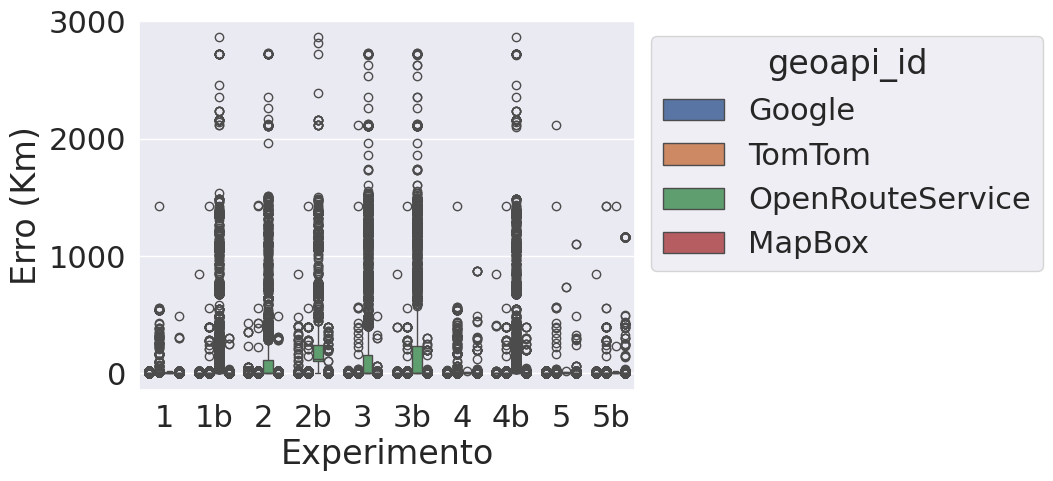
\includegraphics[width=\textwidth]{Figuras/boxplotExperimento.png}
%     \caption{Boxplot de Experimentos por Erro, com todas as APIs avaliadas}
%     \label{fig:boxplot-completo-bh}
% \end{figure}

% Consequentemente, geramos o boxplot sem outliers, representado na Figura \ref{fig:boxplot-semout-bh}. Nela, conseguimos observar claramente o desempenho da ORS, que obteve os piores resultados. Os erros da ORS, sem outliers, ultrapassam 400 km, apesar do boxplot estar contido na faixa de 200 km. De qualquer forma, a presença da ORS prejudica a comparação com as outras APIs, que era o objetivo inicial na criação desses boxplots.

% \begin{figure}[h]
%     \centering
%     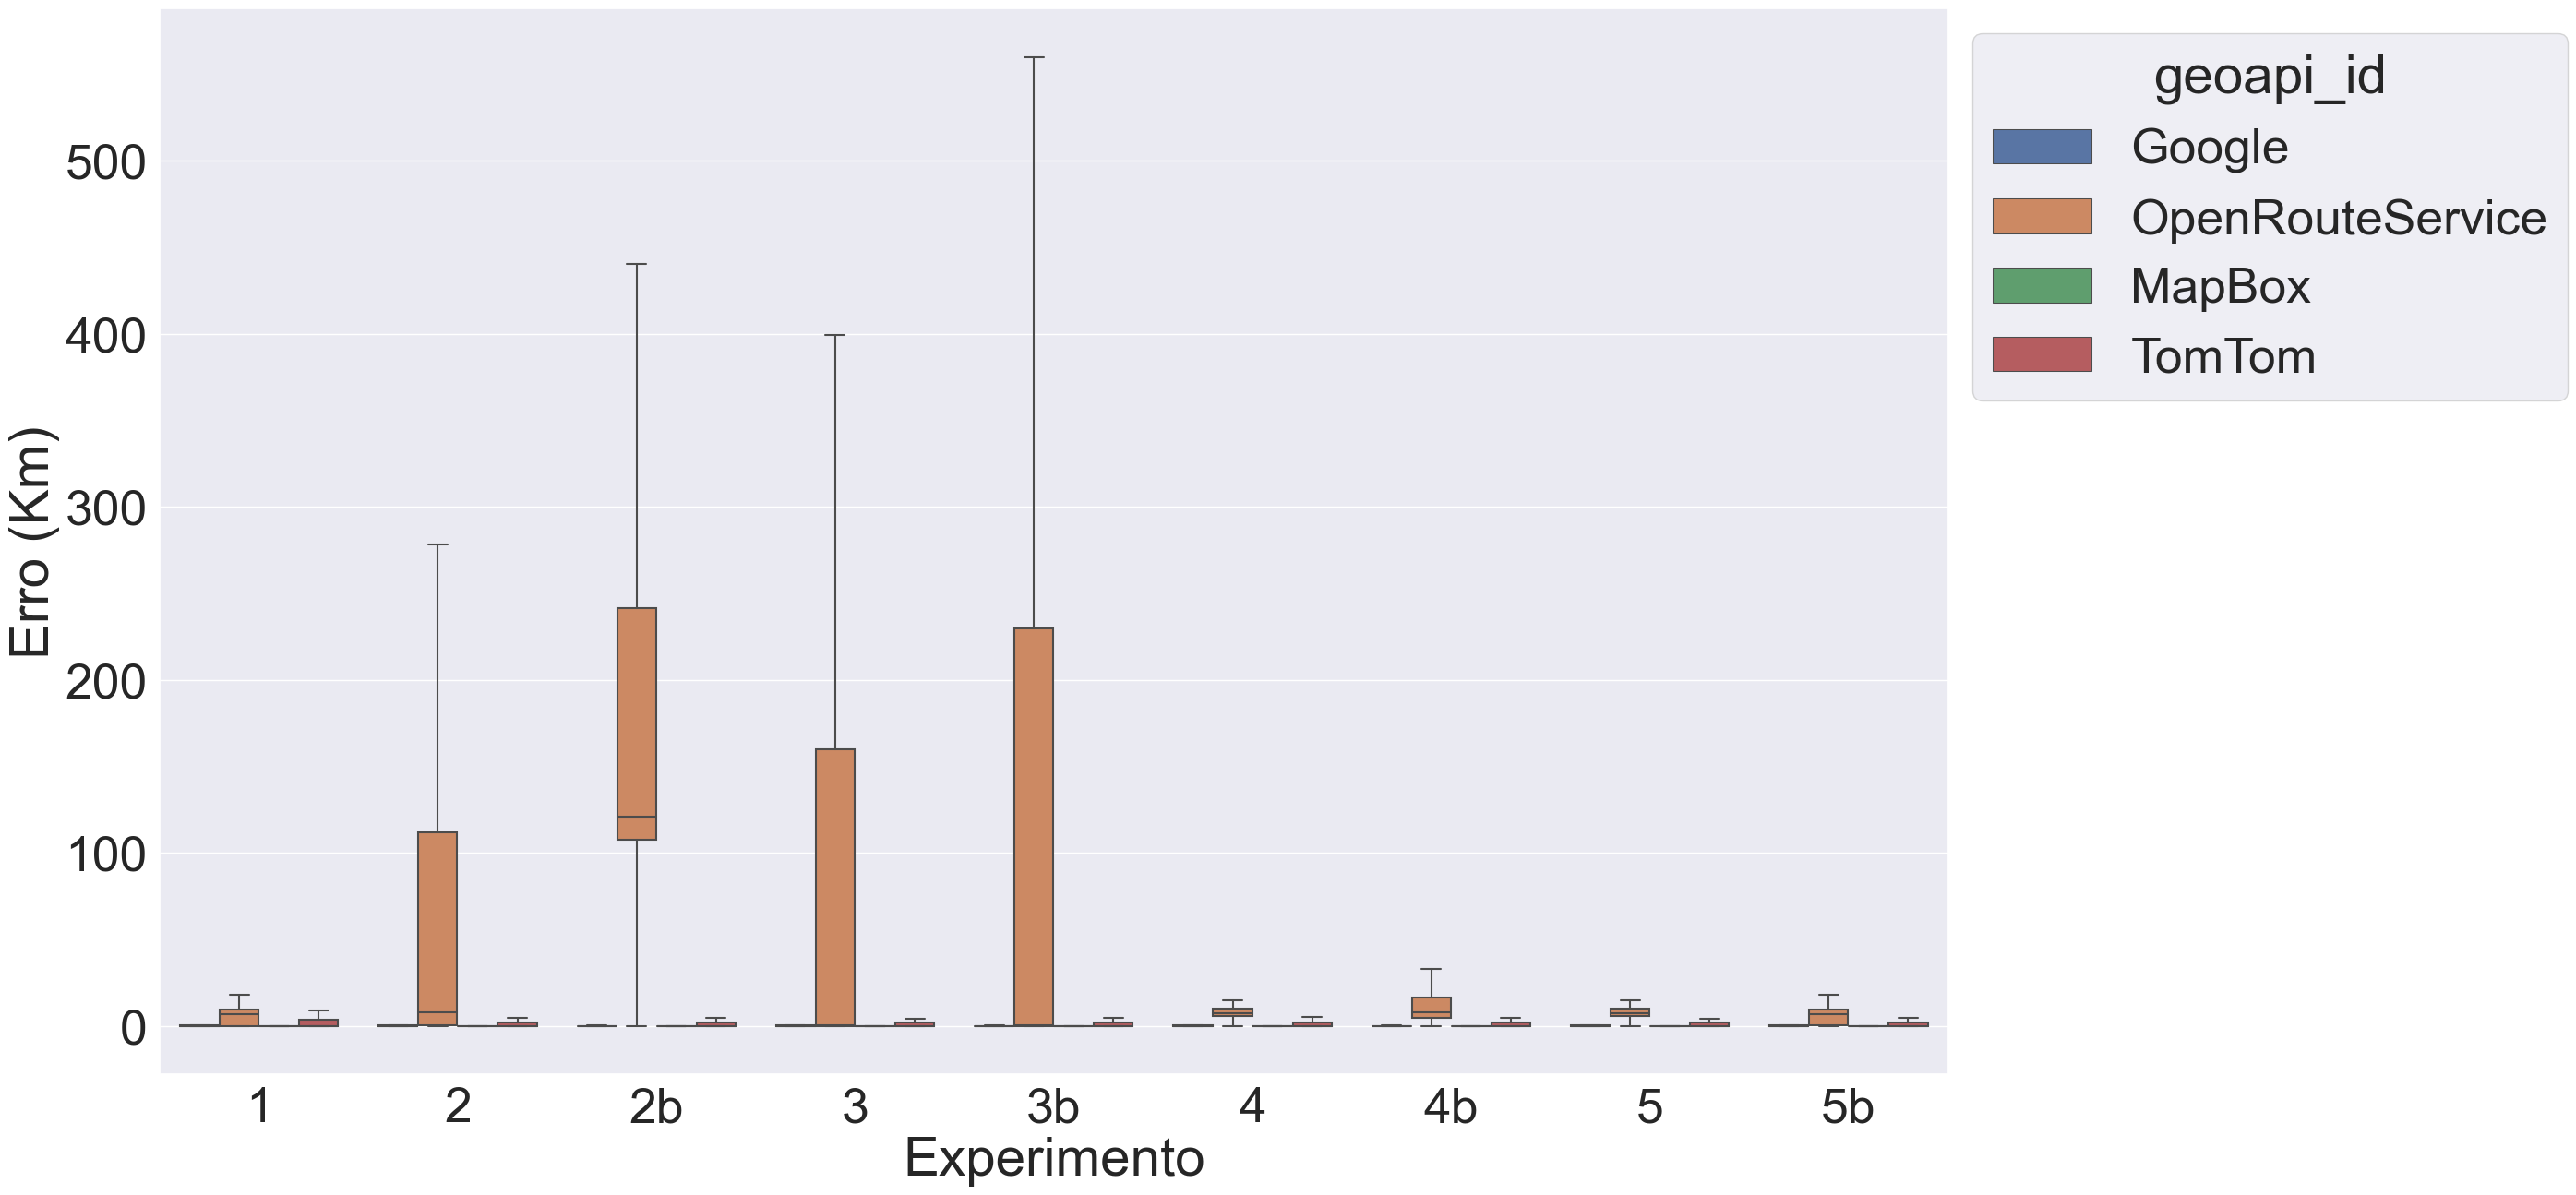
\includegraphics[width=\textwidth]{Figuras/boxplotExperimentoSemOut.png}
%     \caption{Boxplot de Experimentos por Erro, com todas as APIs avaliadas e sem Outliers}
%     \label{fig:boxplot-semout-bh}
% \end{figure}

% %\begin{figure}[h]
% %    \centering
% %    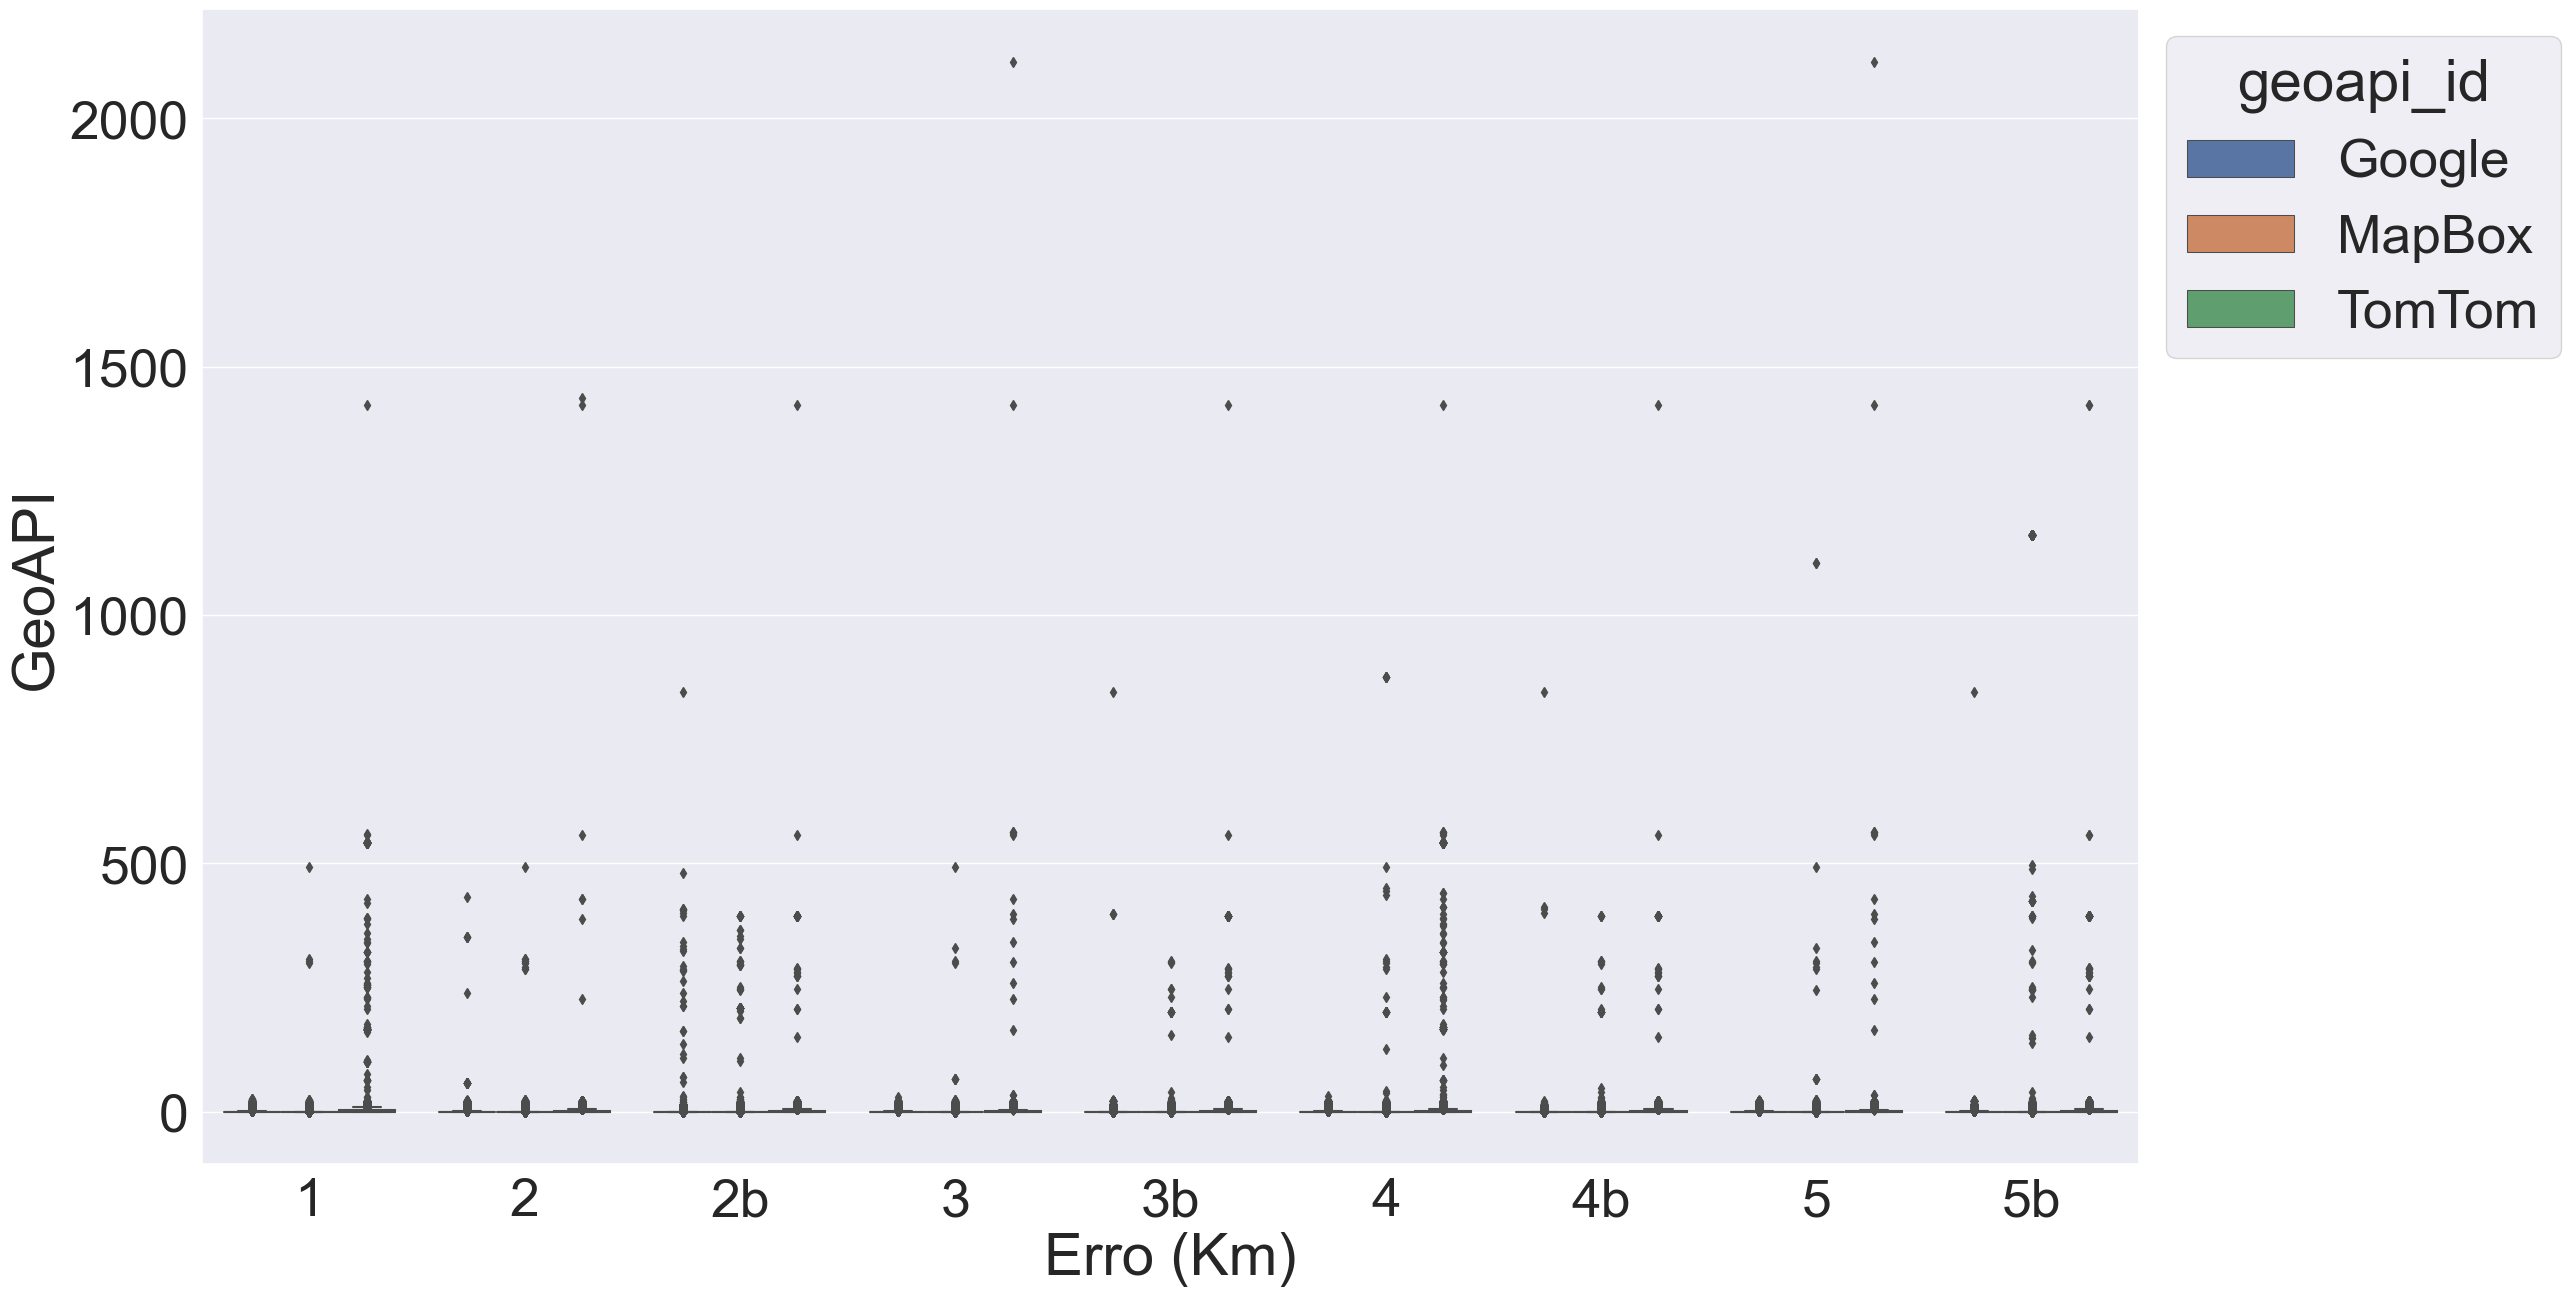
\includegraphics[width=\textwidth]{Figuras/boxplotExperimentoSemORS.png}
% %    \caption{Boxplot de Experimentos por Erro, com todas as APIs avaliadas exceto ORS}
% %    \label{fig:boxplot-semors-bh}
% %\end{figure}

% Decidimos então criar um boxplot que não contivesse dados da ORS, como mostrado na Figura \ref{fig:boxplot-semors-semout-bh}. Nesse gráfico, podemos observar que o erro é limitado a 8 km, um resultado consideravelmente melhor do que os obtidos anteriormente. Além disso, notamos que a API TomTom tem uma barra maior, indicando uma faixa de erro maior, conforme esperado de acordo com a tabela \ref{tab:txAcerExpAPIBH}. Observamos também que as APIs Google e MapBox têm barras de tamanho similar, sendo a MapBox ligeiramente menor. Um ponto interessante é que, ao comparar os experimentos, o destaque é o Experimento 1b, com uma barra menor em todas as APIs. Este experimento segue o código postal brasileiro, mas com a adição de bairro, indicando novamente que essa formatação pode gerar bons resultados para geocodificação.
  
% \begin{figure}[h]
%     \centering
%     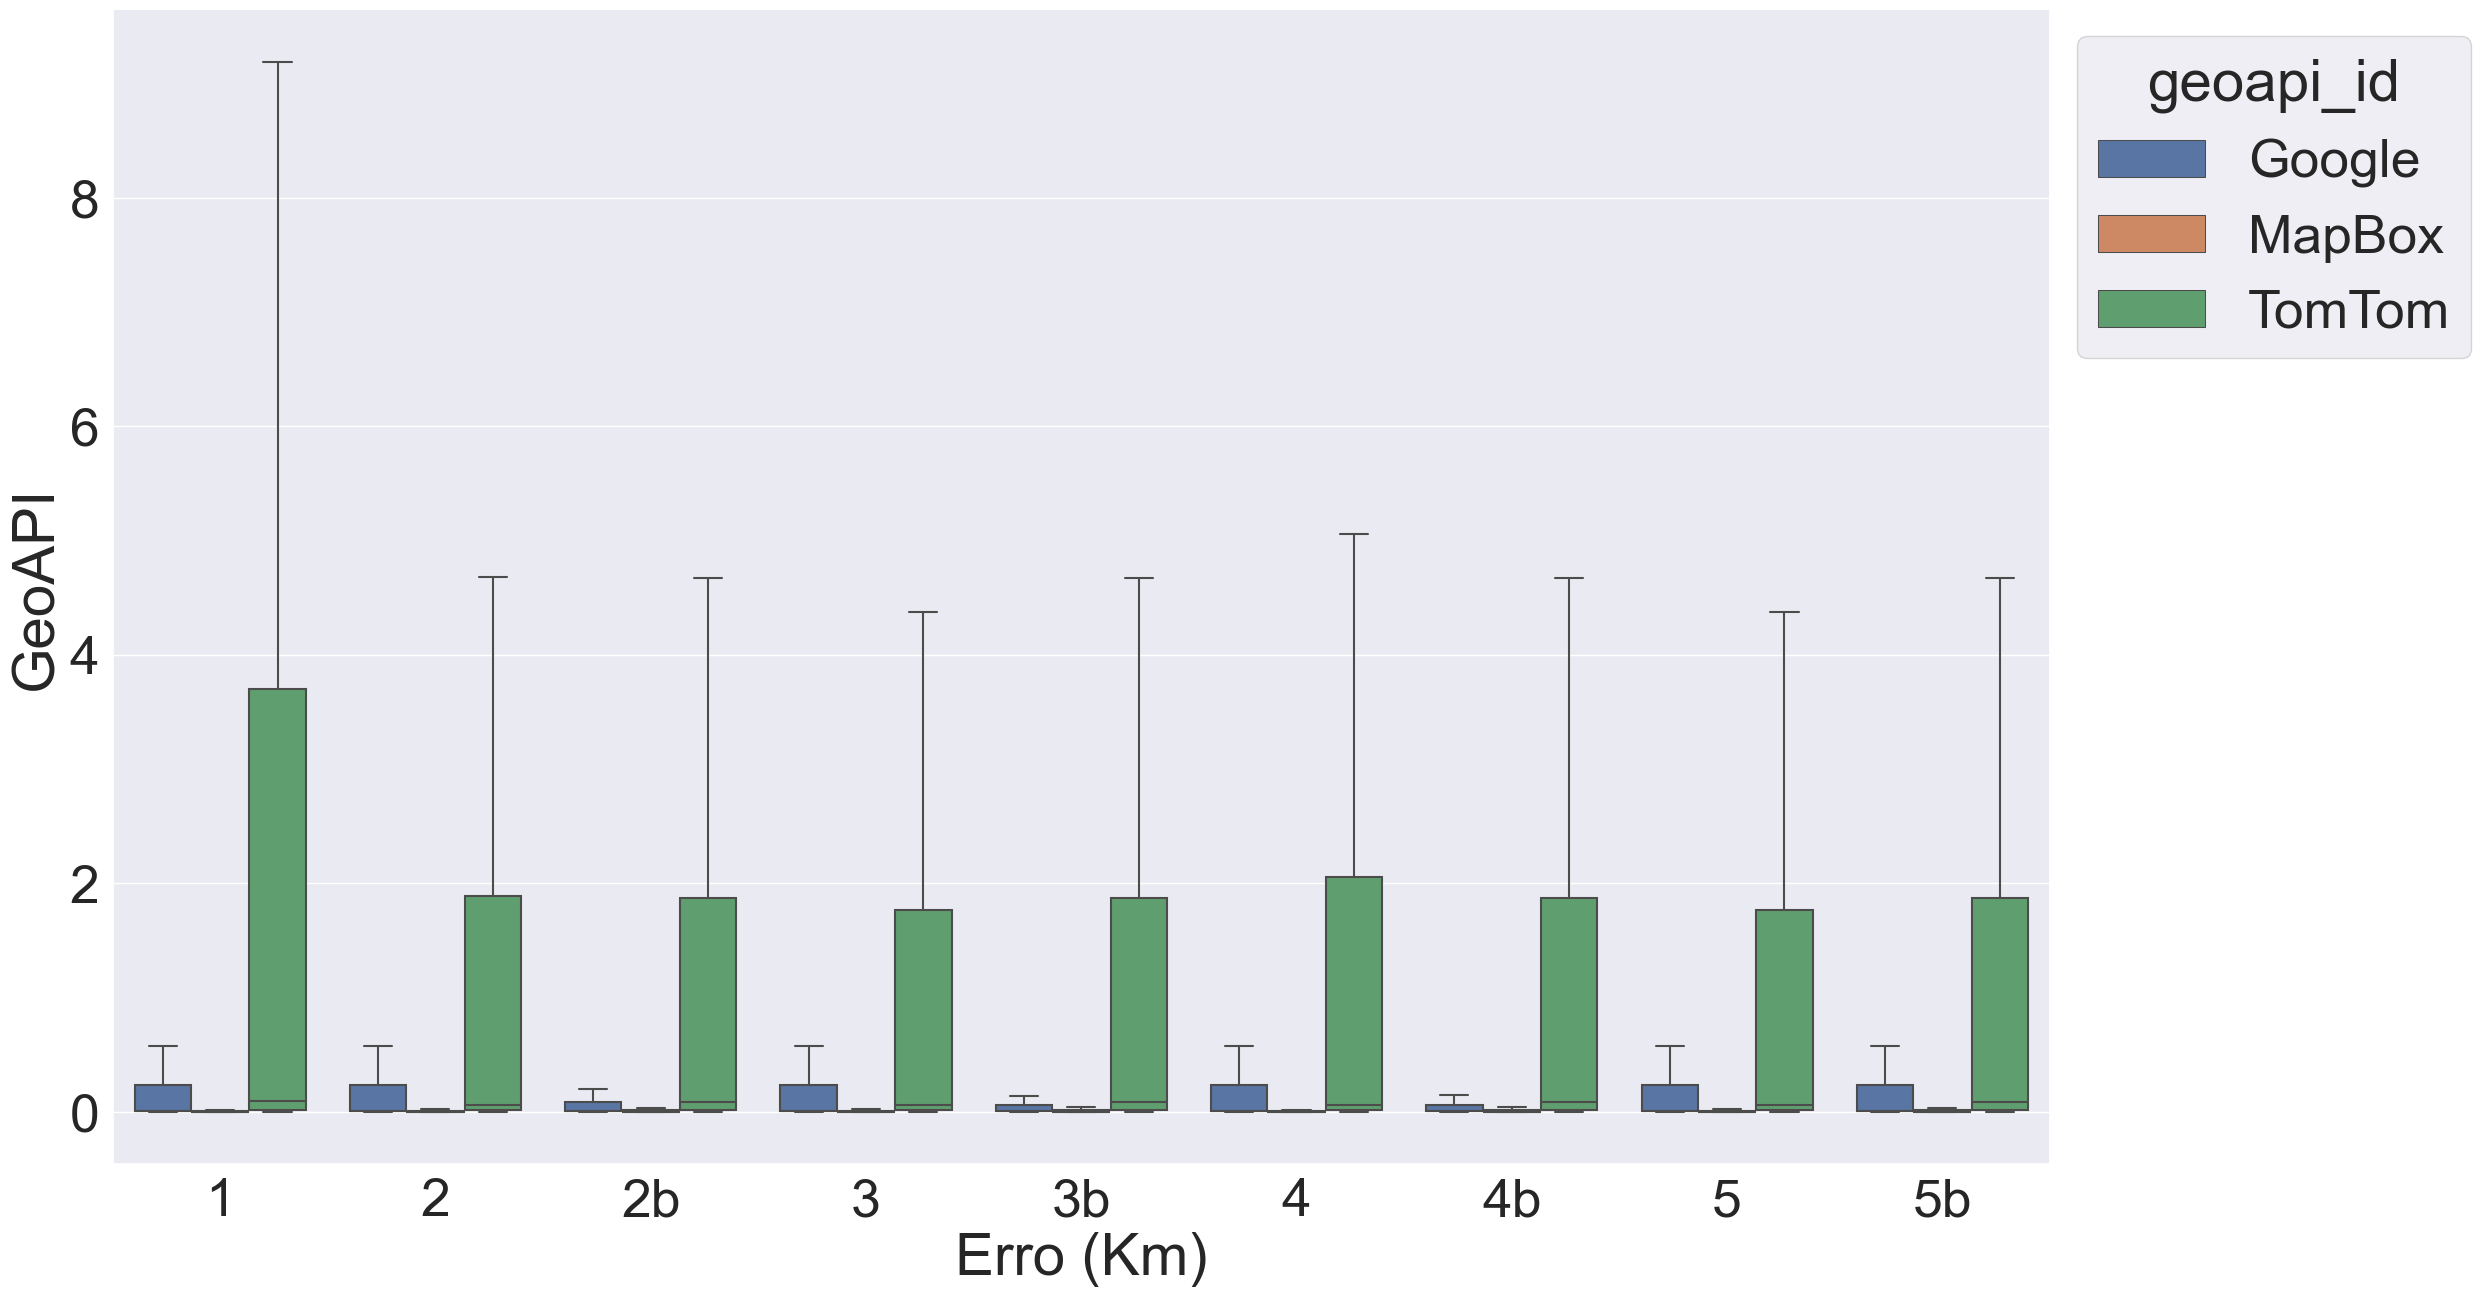
\includegraphics[width=\textwidth]{Figuras/boxplotExperimentoSemOutSemORS.png}
%     \caption{Boxplot de Experimentos por Erro, com todas as APIs avaliadas exceto ORS e sem Outliers}
%     \label{fig:boxplot-semors-semout-bh}
% \end{figure}

% Para a base de São Paulo, foram construídos boxplots de forma semelhante. A Figura \ref{fig:boxplot-completo-sp} mostra o boxplot de experimento por erro com todas as APIs, sem remover os outliers. Assim como nos dados de Belo Horizonte, esse boxplot fornece pouca informação útil. É possível observar que, mais uma vez, o erro atinge a faixa de 3.000 km e que a ORS tem uma faixa de erro maior. No entanto, não é possível tirar muitas conclusões devido à presença de outliers.

% \begin{figure}[h]
%     \centering
%     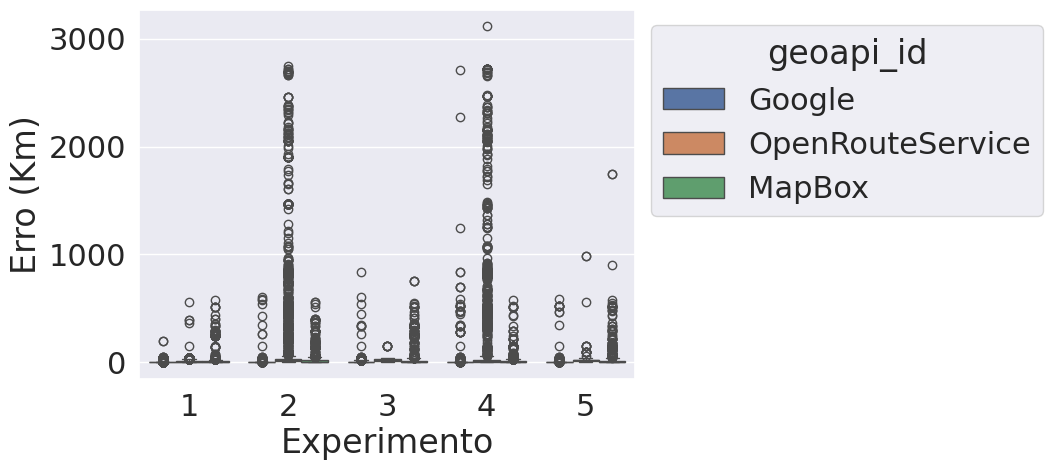
\includegraphics[width=\textwidth]{Figuras/boxplotExperimentoSP.png}
%     \caption{Boxplot de Experimentos por Erro, com todas as APIs avaliadas para a amostra de São Paulo}
%     \label{fig:boxplot-completo-sp}
% \end{figure}

% Posteriormente, geramos boxplots sem outliers. A Figura \ref{fig:boxplot-semout-sp} mostra esse boxplot. Observamos que a ORS teve o pior resultado, mas, ao contrário do boxplot \ref{fig:boxplot-semout-bh}, ainda é possível distinguir os boxplots das outras APIs. Ou seja, o desempenho da ORS não foi tão discrepante como o de Belo Horizonte. Outro ponto importante é que neste boxplot é possível perceber uma grande diferença entre a Google e a Mapbox, com a Google obtendo resultados consideravelmente melhores. Em relação aos experimentos, o Experimento 1 foi o que obteve os melhores resultados. Novamente, o Experimento 1 segue o padrão do código postal do Brasil, o que parece confirmar a hipótese de que essa é a melhor formatação de entrada.


% \begin{figure}[h]
%     \centering
%     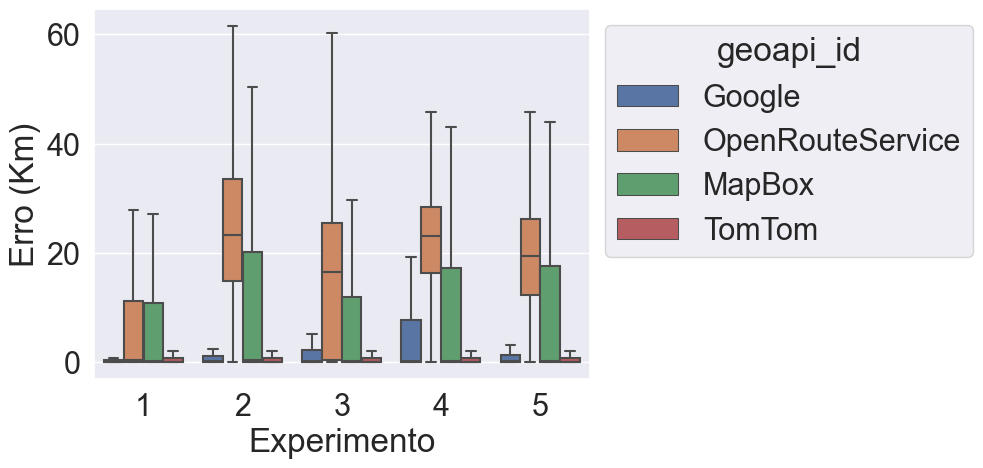
\includegraphics[width=\textwidth]{Figuras/boxplotExperimentoSemOutSP.png}
%     \caption{Boxplot de Experimentos por Erro, com todas as APIs avaliadas e sem Outliers para a amostra de São Paulo}
%     \label{fig:boxplot-semout-sp}
% \end{figure}

% %\begin{figure}[h]
% %    \centering
% %    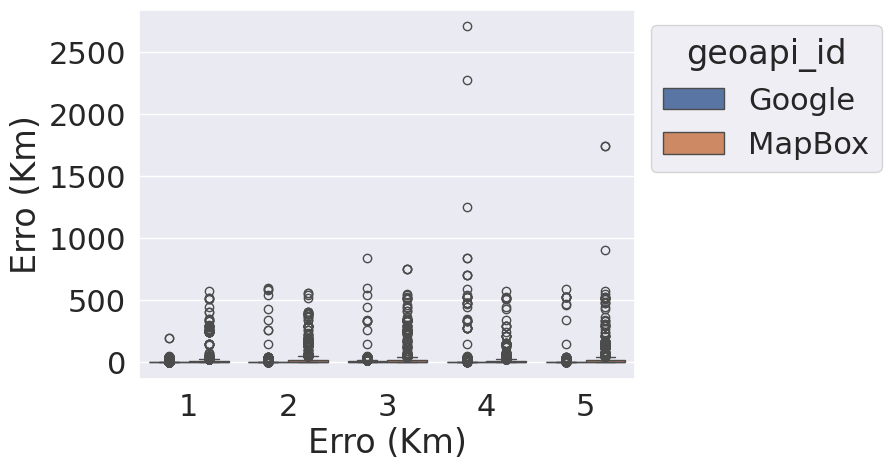
\includegraphics[width=\textwidth]{Figuras/boxplotExperimentoSemORSSP.png}
% %    \caption{Boxplot de Experimentos por Erro, com todas as APIs avaliadas exceto ORS para a amostra de São Paulo}
% %    \label{fig:boxplot-semors-sp}
% %\end{figure}

% %\begin{figure}[h]
% %    \centering
% %    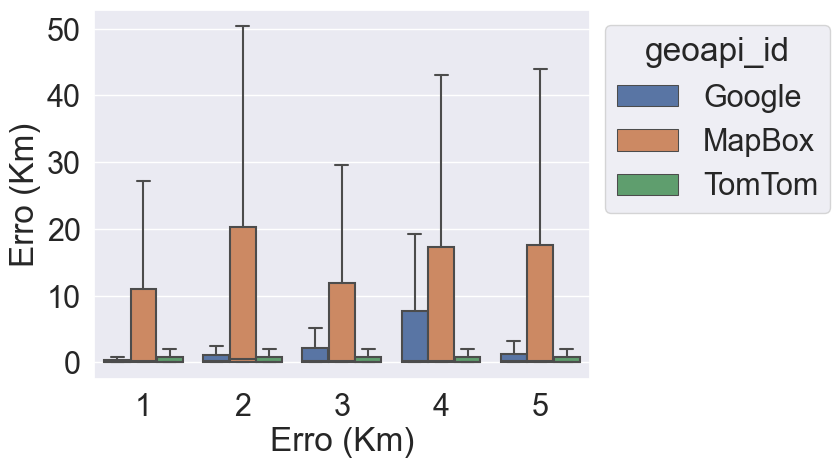
\includegraphics[width=\textwidth]{Figuras/boxplotExperimentoSemOutSemORSSP.png}
% %    \caption{Boxplot de Experimentos por Erro, com todas as APIs avaliadas exceto ORS e sem Outliers para a amostra de São Paulo}
% %    \label{fig:boxplot-semors-semout-sp}
% %\end{figure}

% Os boxplots apresentados anteriormente foram cruciais para avaliar as APIs comparativamente. No entanto, faltava avaliar o comportamento dos experimentos dentro de cada API. Para isso, foram criados boxplots para cada API, onde o boxplot representa o experimento. As Figuras \ref{fig:boxplot-api-global-bh} e \ref{fig:boxplot-api-global-sp} mostram os boxplots de Belo Horizonte e São Paulo, respectivamente. Assim como nos boxplots anteriores, a presença de outliers prejudica a visualização, mas ainda é possível observar a faixa de erro em cada API. Abaixo, são apresentados os valores máximos de erro:

% \begin{itemize}
%   \item MapBox - Belo Horizonte: Acima de 1000 km;
%   \item Google - Belo Horizonte: Acima de 800 km;
%   \item TomTom - Belo Horizonte: Acima de 2000 km;
%   \item ORS - Belo Horizonte: Acima de 1000 km;
%   \item MapBox - São Paulo: Acima de 1500 km;
%   \item Google - São Paulo: Acima de 2500 km;
%   \item ORS - São Paulo: Acima de 3000 km;
% \end{itemize} 


% \begin{figure}[ht]
%   \centering
%   \begin{subfigure}[b]{0.45\textwidth}
%     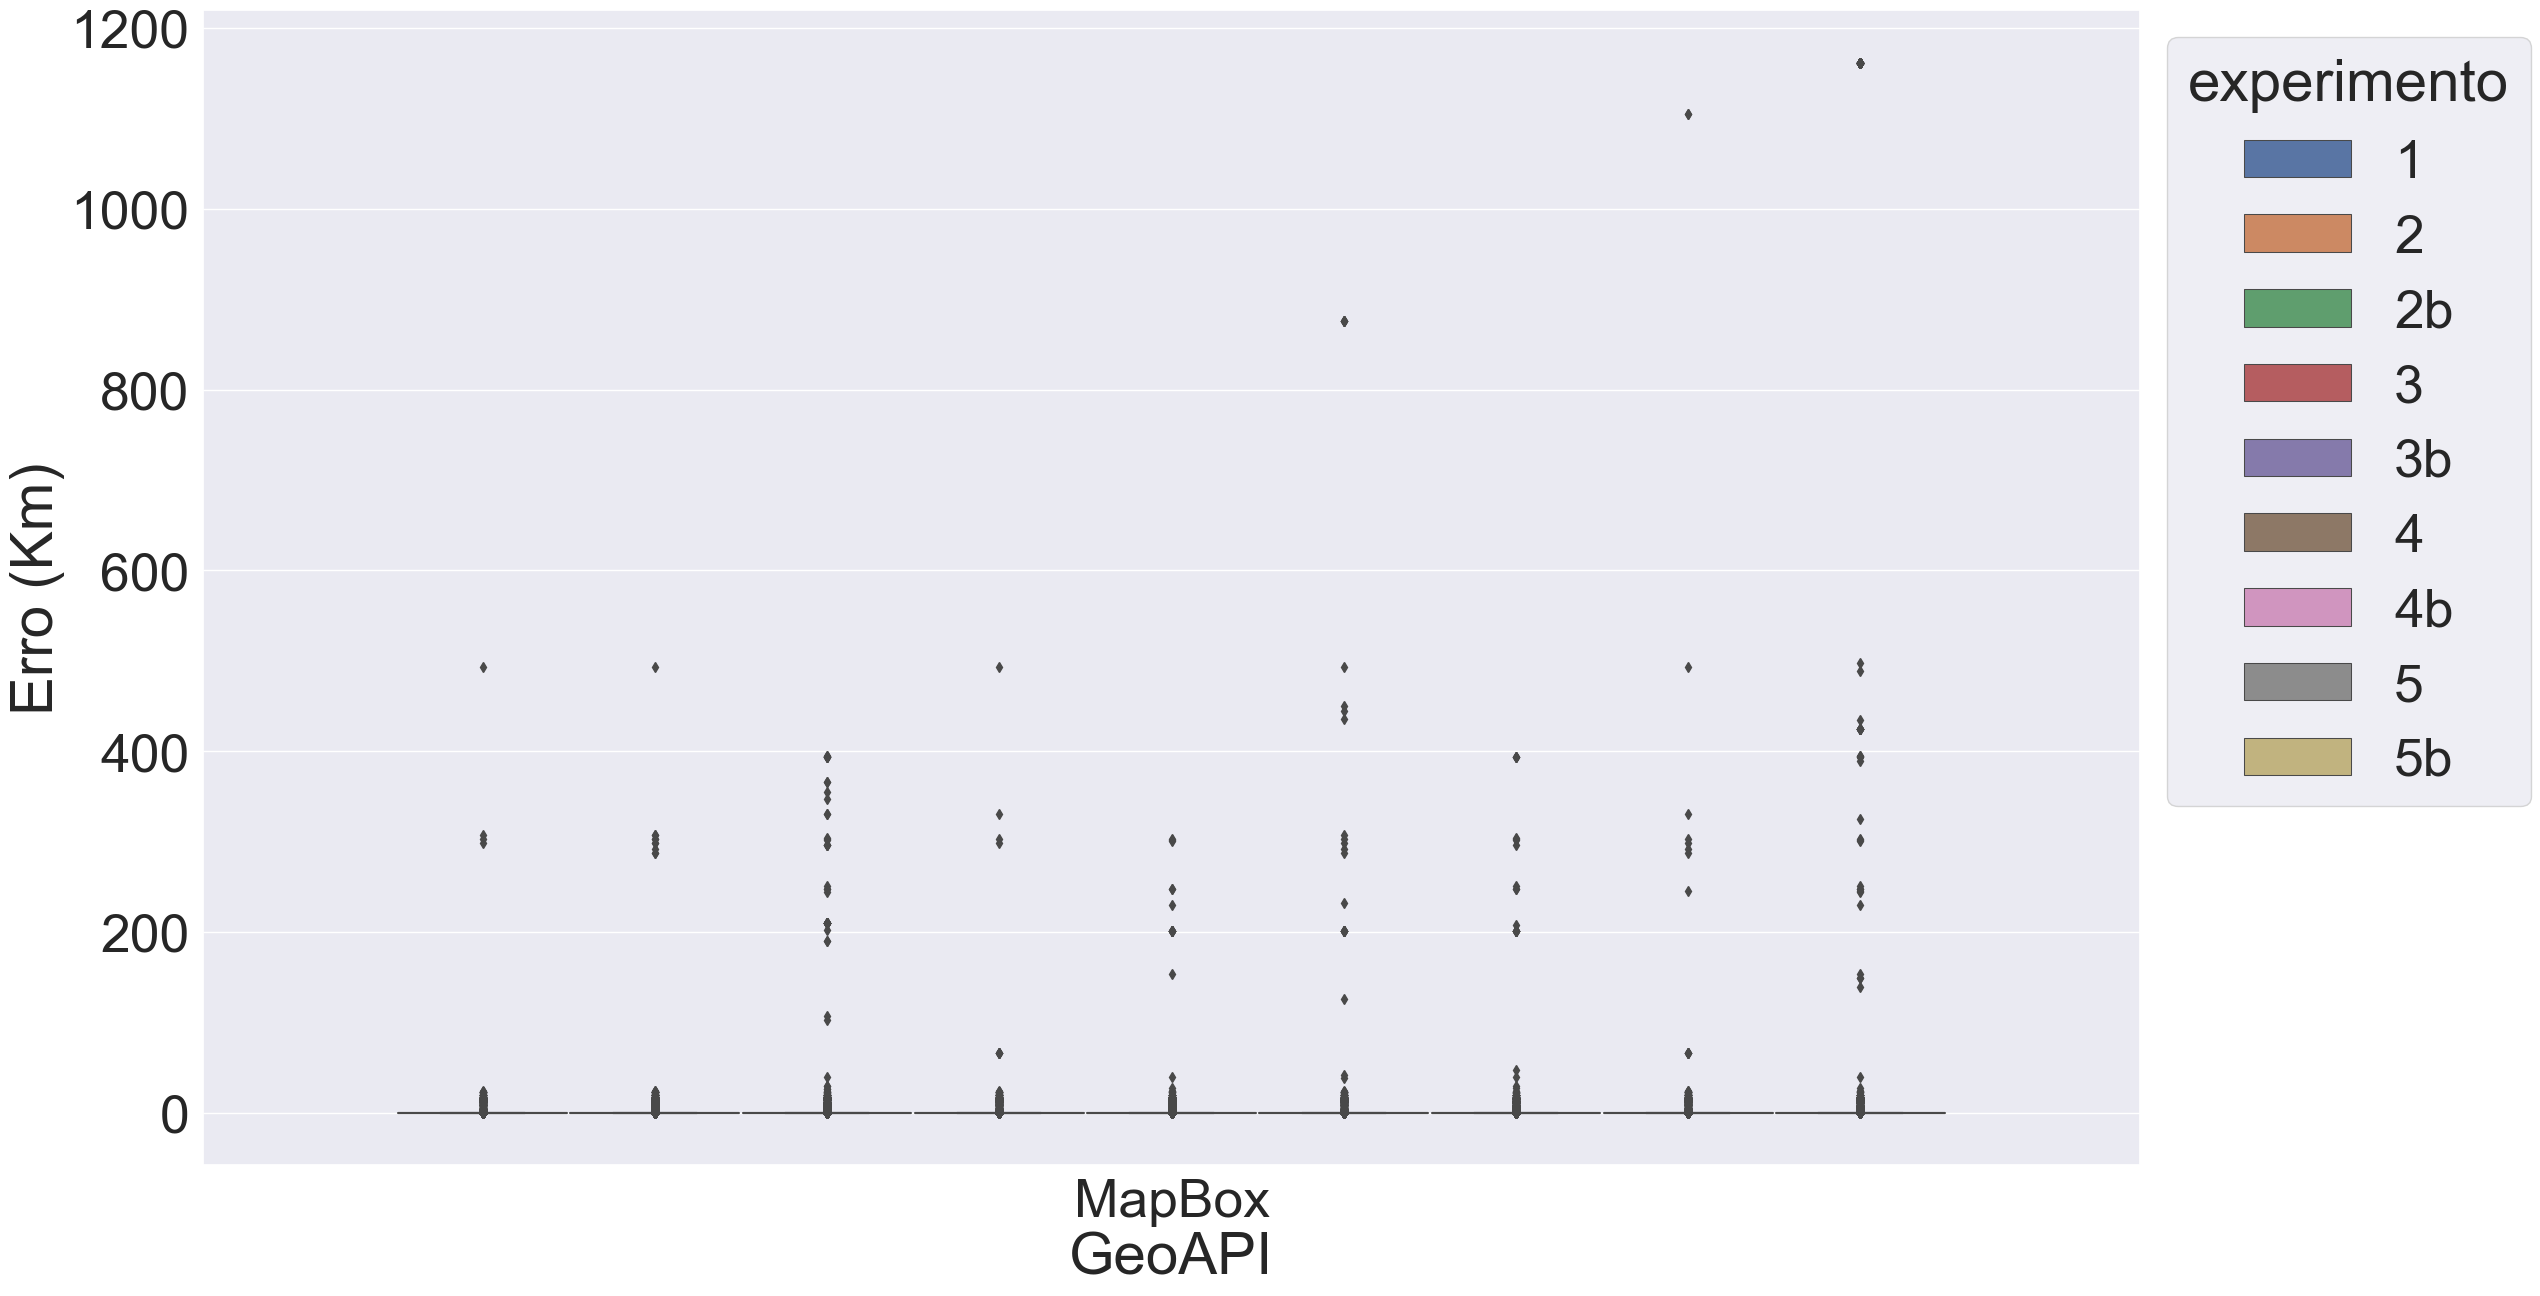
\includegraphics[width=\textwidth]{Figuras/boxplotApiMapbox.png}
%     \caption{Mapbox}
%     \label{fig:boxplot-api-mapbox}
%   \end{subfigure}
%   \hfill
%   \begin{subfigure}[b]{0.45\textwidth}
%     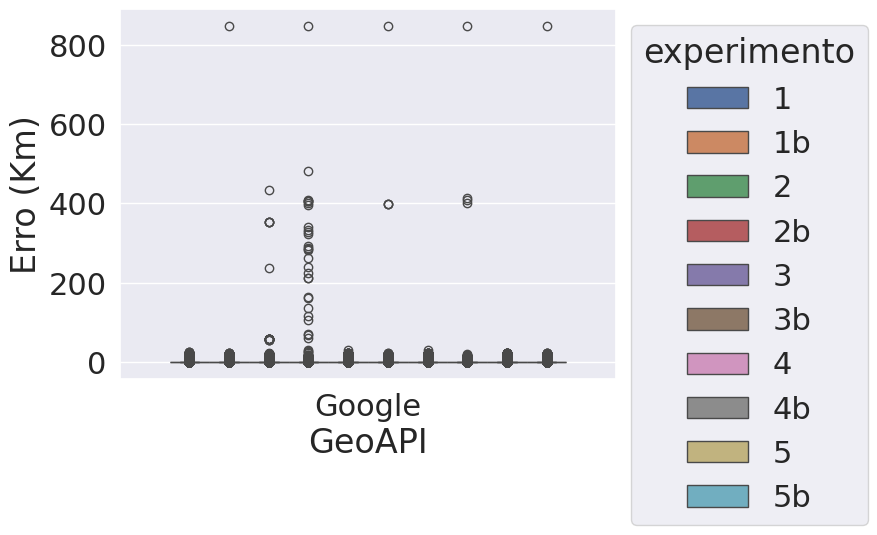
\includegraphics[width=\textwidth]{Figuras/boxplotApiGoogle.png}
%     \caption{Google}
%     \label{fig:boxplot-api-google}
%   \end{subfigure}

%   \begin{subfigure}[b]{0.45\textwidth}
%     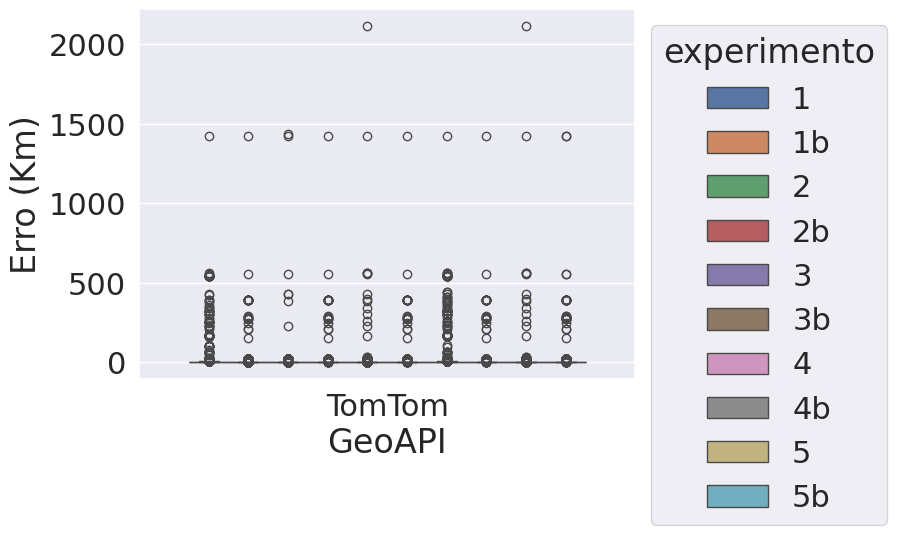
\includegraphics[width=\textwidth]{Figuras/boxplotApiTomtom.png}
%     \caption{TomTom}
%     \label{fig:boxplot-api-tomtom}
%   \end{subfigure}
%   \hfill
%   \begin{subfigure}[b]{0.45\textwidth}
%     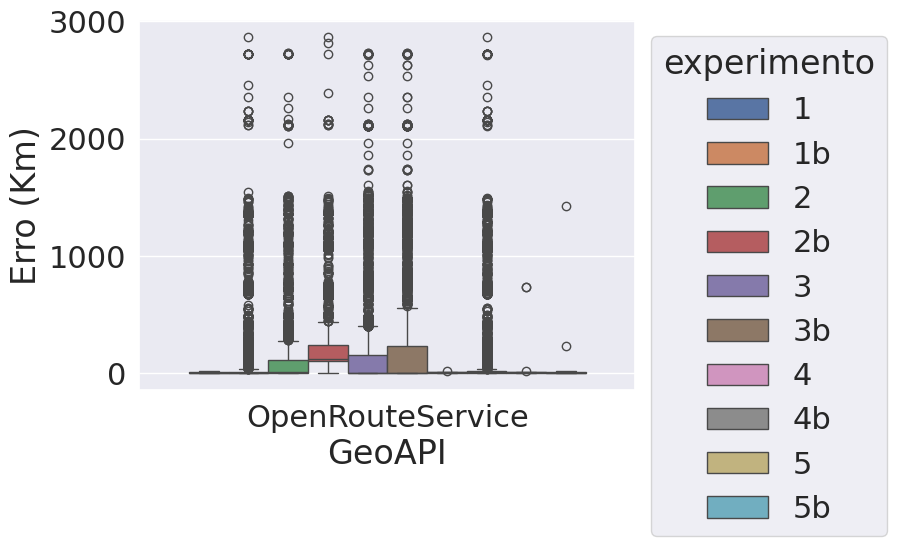
\includegraphics[width=\textwidth]{Figuras/boxplotApiOrs.png}
%     \caption{ORS}
%     \label{fig:boxplot-api-ors}
%   \end{subfigure}
  
%   \caption{Boxplots de Erro por API para cada uma das APIs avalidas}
%   \label{fig:boxplot-api-global-bh}
% \end{figure}

% \begin{figure}[ht]
%   \centering
%   \begin{subfigure}[b]{0.45\textwidth}
%     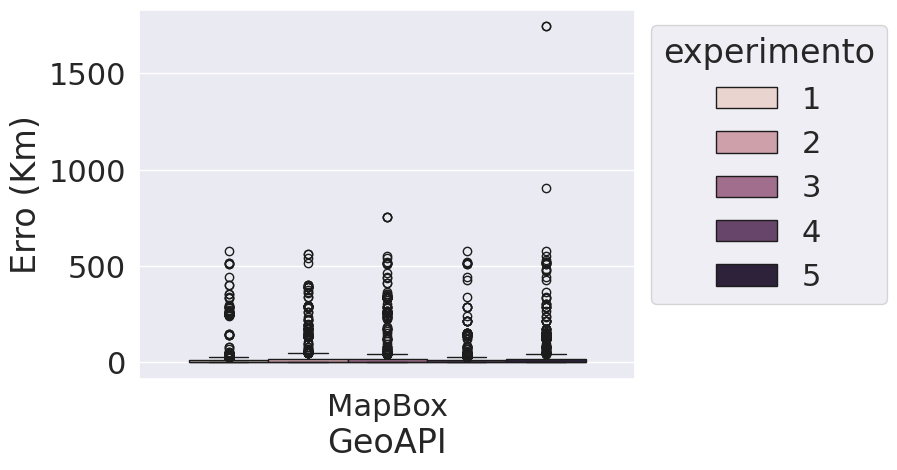
\includegraphics[width=\textwidth]{Figuras/boxplotApiMapboxSP.png}
%     \caption{Mapbox}
%     \label{fig:boxplot-api-mapbox-sp}
%   \end{subfigure}
%   \hfill
%   \begin{subfigure}[b]{0.45\textwidth}
%     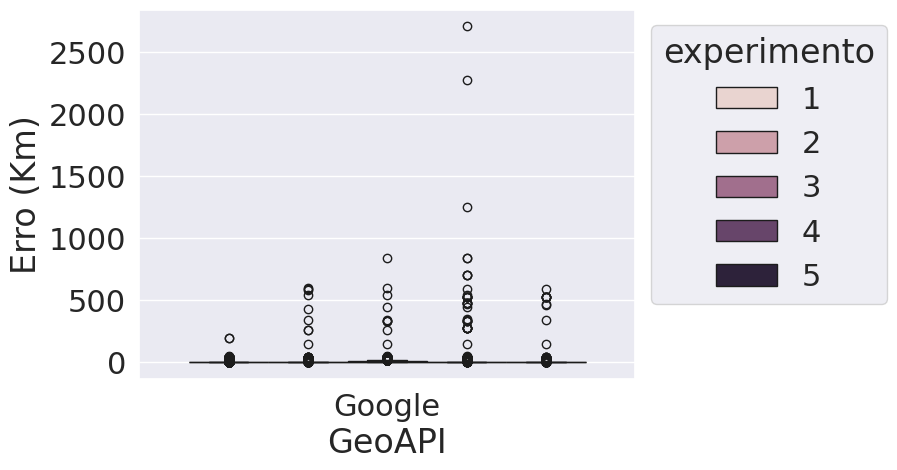
\includegraphics[width=\textwidth]{Figuras/boxplotApiGoogleSP.png}
%     \caption{Google}
%     \label{fig:boxplot-api-google-sp}
%   \end{subfigure}
  
%   \begin{subfigure}[b]{0.45\textwidth}
%     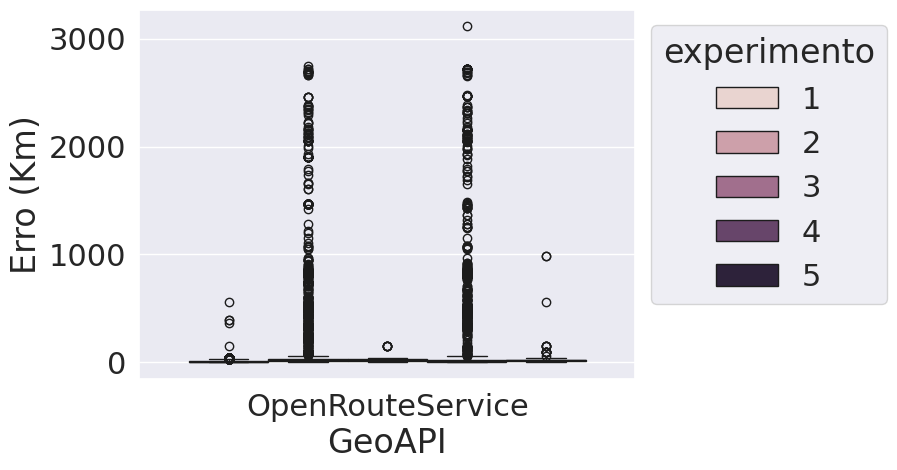
\includegraphics[width=\textwidth]{Figuras/boxplotApiOrsSP.png}
%     \caption{ORS}
%     \label{fig:boxplot-api-ors-sp}
%   \end{subfigure}
  
%   \caption{Boxplots de Erro por API para cada uma das APIs avalidas para a amostra de São Paulo}
%   \label{fig:boxplot-api-global-sp}
% \end{figure}

% Para aprimorar a visualização, decidimos remover os outliers de todos os boxplots.

% As Figuras \ref{fig:boxplot-api-mapbox-semout-bh} e \ref{fig:boxplot-api-mapbox-semout-sp} apresentam os boxplots do erro da Mapbox para os dados de Belo Horizonte e São Paulo, respectivamente. Em ambos os boxplots, o Experimento 1 obteve os melhores resultados para a API MapBox. No entanto, é interessante observar que o Experimento 4 teve um desempenho muito semelhante ao Experimento 1 para ambas as bases. Analisando o boxplot de Belo Horizonte, é possível notar que a adição do bairro resultou em piora nos resultados para todos os experimentos, evidenciando os piores resultados em geral, conforme observado na tabela \ref{tab:txAcerExpAPIBH}. Quanto aos dados de São Paulo, os experimentos que se destacaram negativamente foram o 2, 3 e 5.

% \begin{figure}[h]
%     \centering
%     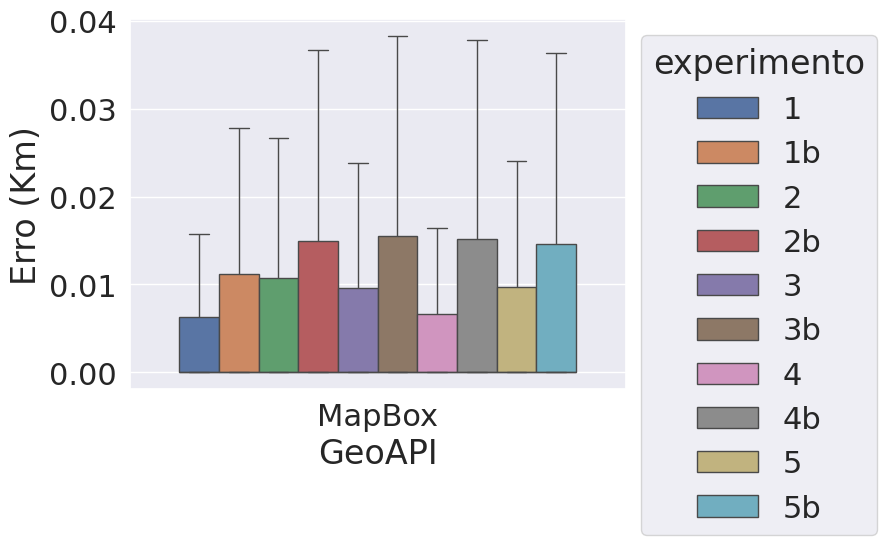
\includegraphics[width=\textwidth]{Figuras/boxplotApiMapboxSemOut.png}
%     \caption{Boxplot de Erro por API com todos os experimentos avaliados sem Outliers: Mapbox}
%     \label{fig:boxplot-api-mapbox-semout-bh}
% \end{figure}

% \begin{figure}[h]
%   \centering
%   \includegraphics[width=\textwidth]{Figuras/boxplotApiMapboxSemOutsp.png}
%   \caption{Boxplot de Erro por API com todos os experimentos avaliados sem Outliers para a amostra de São Paulo: Mapbox}
%   \label{fig:boxplot-api-mapbox-semout-sp}
% \end{figure}

% As Figuras \ref{fig:boxplot-api-google-semout-bh} e \ref{fig:boxplot-api-google-semout-sp} apresentam os boxplots referentes aos dados de Belo Horizonte e São Paulo, respectivamente. Ao analisar os dados de Belo Horizonte, observa-se uma melhora considerável em quase todos os experimentos nos casos em que o bairro foi adicionado. A exceção são os experimentos 5 e 5b, nos quais a diferença não é significativa. O experimento com melhor desempenho para os dados de Belo Horizonte foi o experimento 1b, enquanto para os dados de São Paulo, o destaque foi para o experimento 1. Esses resultados confirmam as conclusões extraídas das tabelas \ref{tab:txAcerExpAPIBH} e \ref{tab:txAcerExpAPISP}, indicando que essa formatação é a mais eficaz.

% Quanto aos piores resultados, para os dados de Belo Horizonte, as performances mais baixas foram observadas nos casos em que não havia informação de bairro, sem diferenças significativas entre eles. Já para os dados de São Paulo, a pior performance foi no experimento 3.


% \begin{figure}[h]
%     \centering
%     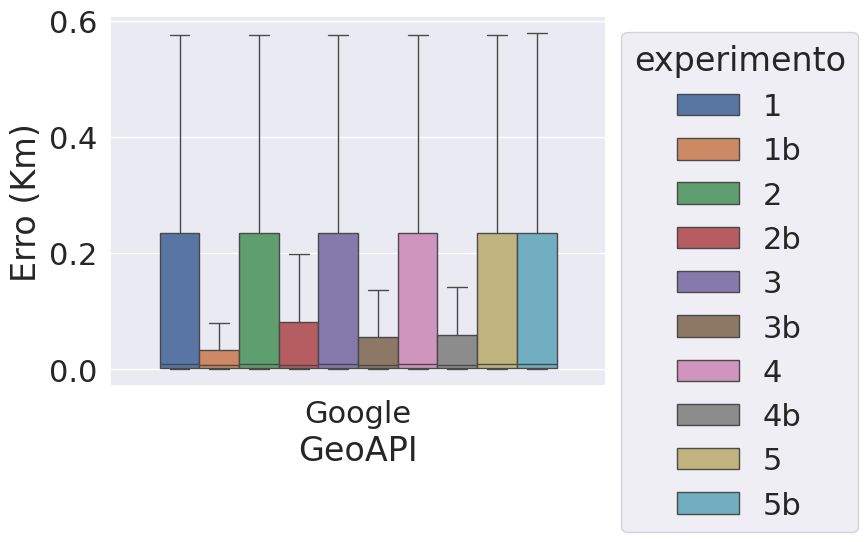
\includegraphics[width=\textwidth]{Figuras/boxplotApiGoogleSemOut.png}
%     \caption{Boxplot de Erro por API com todos os experimentos avaliados sem Outliers: Google}
%     \label{fig:boxplot-api-google-semout-bh}
% \end{figure}


% \begin{figure}[h]
%   \centering
%   \includegraphics[width=\textwidth]{Figuras/boxplotApiGoogleSemOutsp.png}
%   \caption{Boxplot de Erro por API com todos os experimentos avaliados sem Outliers para a amostra de São Paulo: Google}
%   \label{fig:boxplot-api-google-semout-sp}
% \end{figure}

% A Figura \ref{fig:boxplot-api-tomtom-semout-bh} apresenta o boxplot da API TomTom para os dados de Belo Horizonte. Observa-se que o experimento com melhor desempenho foi o 1b, enquanto o pior desempenho ocorreu no experimento 1, contrariando os resultados previamente obtidos. Os demais experimentos apresentaram resultados semelhantes, e não é possível afirmar que há uma melhora ao adicionar o bairro nesses experimentos, exceto nos casos do experimento 1 e 1b, nos quais houve uma melhora significativa ao adicionar o bairro.

% \begin{figure}[h]
%     \centering
%     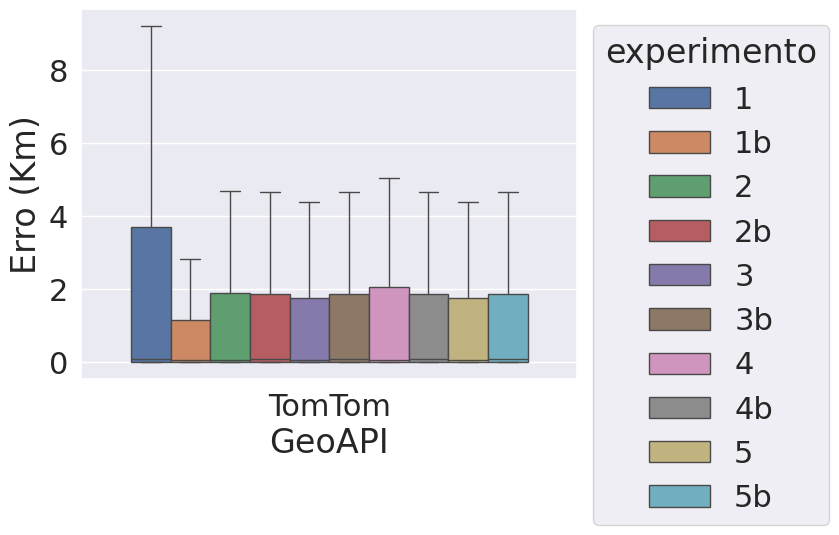
\includegraphics[width=\textwidth]{Figuras/boxplotApiTomtomSemOut.png}
%     \caption{Boxplot de Erro por API com todos os experimentos avaliados sem Outliers: TomTom}
%     \label{fig:boxplot-api-tomtom-semout-bh}
% \end{figure}

% Para concluir a análise dos boxplots, foram gerados dois gráficos para os dados de Belo Horizonte, conforme apresentado na Figura \ref{fig:boxplot-api-ors-semout-bhe}, e para os dados de São Paulo, na Figura \ref{fig:boxplot-api-ors-semout-sp}. Ao examinar os dados de Belo Horizonte, observa-se que os experimentos que se destacaram positivamente foram os 1, 1b, 4, 4b, 5 e 5b, com pouca diferença entre eles. Por outro lado, os experimentos 2b e 3b obtiveram os piores resultados para os dados de Belo Horizonte. No contexto dos dados de São Paulo, o experimento 1 se destacou positivamente, enquanto o experimento 2 teve o pior desempenho. Os demais experimentos apresentaram resultados semelhantes.


% \begin{figure}[h]
%     \centering
%     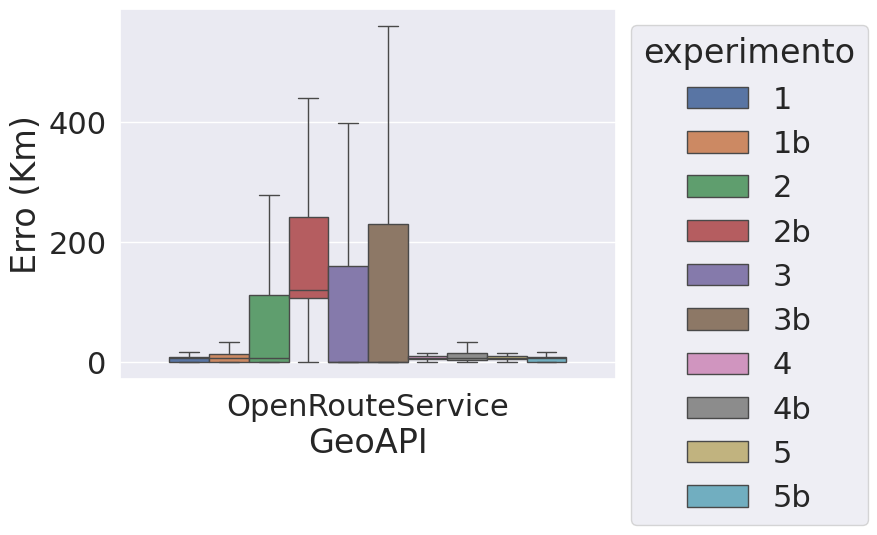
\includegraphics[width=\textwidth]{Figuras/boxplotApiOrsSemOut.png}
%     \caption{Boxplot de Erro por API com todos os experimentos avaliados sem Outliers: ORS}
%     \label{fig:boxplot-api-ors-semout-bh}
% \end{figure}

% \begin{figure}[h]
%     \centering
%     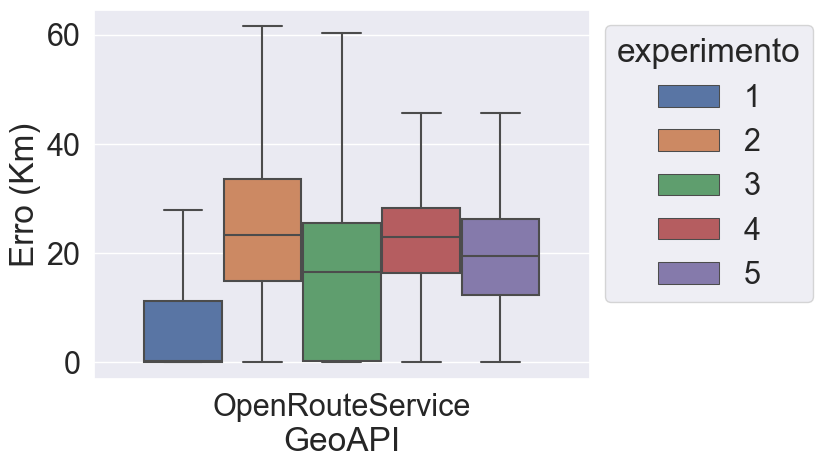
\includegraphics[width=\textwidth]{Figuras/boxplotApiOrsSemOutSP.png}
%     \caption{Boxplot de Erro por API com todos os experimentos avaliados sem Outliers para a amostra de São Paulo: ORS}
%     \label{fig:boxplot-api-ors-semout-sp}
% \end{figure}

% \subsection{Distribuição Espacial das Falhas dos Experimentos de Formatação}

% Por fim, realizamos uma análise espacial de falhas para entender de que forma a formatação da entrada pode contribuir para a falha de forma espacial. 
% Para isso, criamos mapas hexagonais de falhas, como feito anteriormente, para cada API. Escolhemos os experimentos com menor e maior taxa de acerto de cada API a fim de visualizar com mais clareza a melhora a partir de formatações diferentes. 

% A figura \ref{fig:falhas-exp-mapbox-bh} mostra os mapas de falhas dos experimentos com menor e maior taxa de acerto para os dados de Belo Horizonte e para a API Mapbox. Nessa figura é possível observar que no mapa de maior taxa de acerto há uma maior uniformidade e a maior parte do gráfico tem taxa de falha inferior a 20\%. Já no gráfico de menor taxa de acerto há menor uniformidade e as regiões variam de taxas mais baixas (menor que 20\%) até taxas mais altas (maior que 80\%). É relevanteobservar também que as taxas de falha maiores aparentam estar em regiões similares como bordas, o que nos faz pensar que a alta taxa de erro é ligada a região e não somente a formatação de entrada. Apesar disso, até nessas regiões com mais erro, é possível observar uma melhora significativa a partir da formatação com melhor resultado. 

% \begin{figure}[ht]
%   \centering
%   \begin{subfigure}[b]{0.45\textwidth}
%     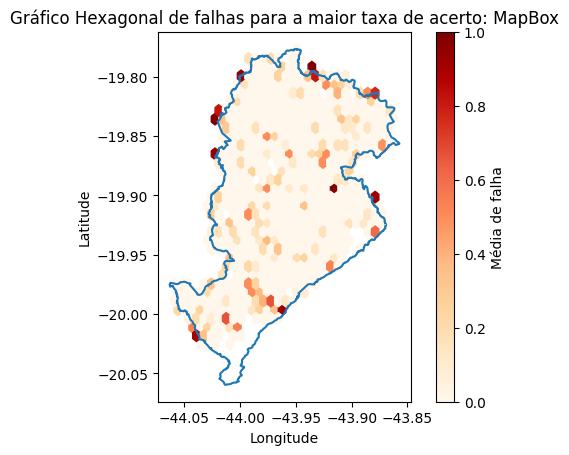
\includegraphics[width=\textwidth]{Figuras/expFalhasMapboxmaior.png}
%     \caption{Maior Taxa de Acerto}
%     \label{fig:falhasmapboxBHexpMaior}
%   \end{subfigure}
%   %\hfill
%   \begin{subfigure}[b]{0.45\textwidth}
%     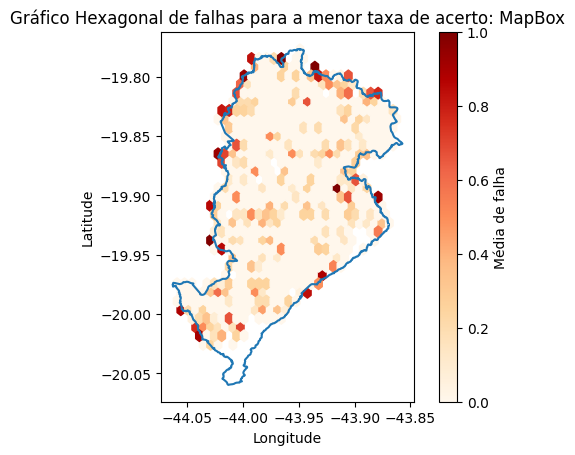
\includegraphics[width=\textwidth]{Figuras/expFalhasMapboxmenor.png}
%     \caption{Menor Taxa de Acerto}
%     \label{fig:falhasmapboxBHexpMenor}
%   \end{subfigure}
  
%   \caption{Gráficos de falhas para a maior e menor taxas de acertodos experimentos para os dados de Belo Horizonte: MapBox}
%   \label{fig:falhas-exp-mapbox-bh}
% \end{figure}

% COLOCAR FALHAS MAPBOX SP

% A figura \ref{fig:falhas-exp-google-bh} mostra os gráficos de falhas para os experimentos de maior e menor taxa de acerto da API Google Maps para os dados de Belo Horizonte. Da mesma forma que acontece nos gráficos da Mapbox, os gráficos para o experimento de maior taxa de acerto apresentam uma uniformidade maior em comparação com o de menor taxa de acerto. Além disso, é interessante observar que existem algumas zonas de onde a taxa de falha é grande em ambos os gráficos. Essas zonas são nas fronteiras da cidade e na parte superior do gráfico. Porém, no gráfico de menor taxa de acerto há uma acentuação dessas regiões com altas taxas de acerto, corroborando com a hipotése de que a formatação realmente contribui para a melhora da taxa de falha. 

% \begin{figure}[ht]
%   \centering
%   \begin{subfigure}[b]{0.45\textwidth}
%     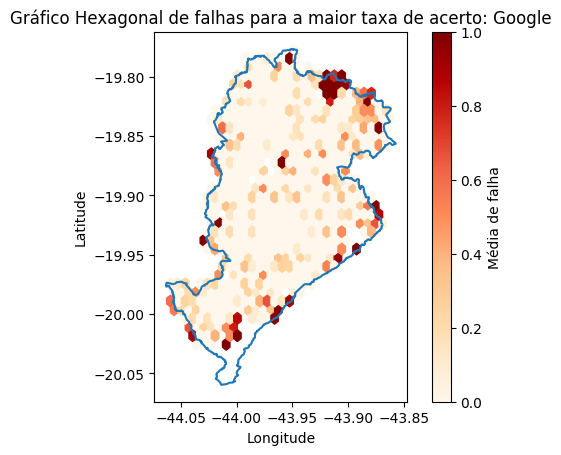
\includegraphics[width=\textwidth]{Figuras/expFalhasGooglemaior.png}
%     \caption{Maior Taxa de Acerto}
%     \label{fig:falhasgoogleBHexpMaior}
%   \end{subfigure}
%   \hfill
%   \begin{subfigure}[b]{0.45\textwidth}
%     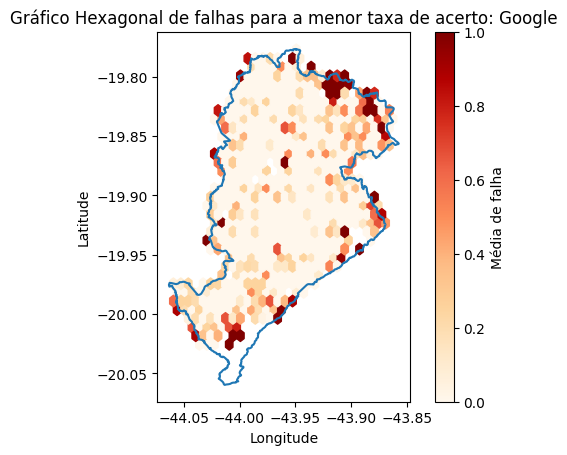
\includegraphics[width=\textwidth]{Figuras/expFalhasGooglemenor.png}
%     \caption{Menor Taxa de Acerto}
%     \label{fig:falhasgoogleBHexpMenor}
%   \end{subfigure}
  
%   \caption{Gráficos de falhas para a maior e menor taxas de acertodos experimentos para os dados de Belo Horizonte: Google Maps}
%   \label{fig:falhas-exp-google-bh}
% \end{figure}

% COLOCAR FALHAS GOOGLE SP

% A figura \ref{fig:falhas-exp-tomtom-bh} mostra os gráficos de falha dos experimentos de maior e menor taxa de acerto da API TomTom para os dados de Belo Horizonte. Nessa figura, ao contrário das outras APIs, não é possível notar diferença significativa entre os experimentos com maior e menor taxa de acerto. Isso condiz com as taxas de acerto da TomTom para os experimentos que estavam todas próximas. Em comparação com as outras APIs, os dois gráficos apresentam uma certa uniformidade, com valores abaixo de 40\% de falha. Algumas regiões aparentam taxas maiores, que são as regiões inferior, superior e de fronteira. Em geral, TomTom apresentou resultados medianos em maior parte dos gráficos. 

% \begin{figure}[ht]
%   \centering
%   \begin{subfigure}[b]{0.45\textwidth}
%     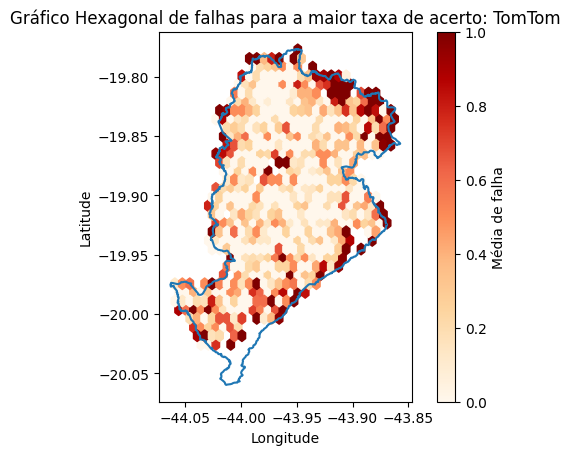
\includegraphics[width=\textwidth]{Figuras/expFalhasTomtommaior.png}
%     \caption{Maior Taxa de Acerto}
%     \label{fig:falhastomtomBHexpMaior}
%   \end{subfigure}
%   \hfill
%   \begin{subfigure}[b]{0.45\textwidth}
%     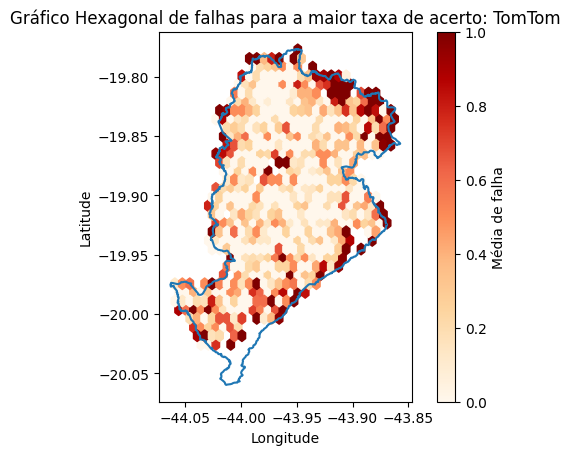
\includegraphics[width=\textwidth]{Figuras/expFalhasTomtommenor.png}
%     \caption{Menor Taxa de Acerto}
%     \label{fig:falhastomtomBHexpMenor}
%   \end{subfigure}
  
%   \caption{Gráficos de falhas para a maior e menor taxas de acertodos experimentos para os dados de Belo Horizonte: TomTom}
%   \label{fig:falhas-exp-tomtom-bh}
% \end{figure}

% COLOCAR FALHAS TOMTOM SP

% A figura \ref{fig:falhas-exp-ors-bh} mostra os gráficos de falha dos experimentos de maior e menor taxa de acerto da API Open Route Service para os dados de Belo Horizonte. Nessa figura, apesar das outras APIs, há pouca uniformiadade no gráfico de maior taxa, inclusive apresentando muitos valores de taxas altas em praticamente todas as regiões do gráfico. Já o gráfico de menor taxa de acerto, apresenta em quase sua totatalidade valores de taxa de acerto próximos do máximo. Ou seja, para a API TomTom, para esses dados, a formatação de entrada é crucial, pois a depender da escolhida, a API pode errar a maioria das solicitações. Apesar disso, mesmo no experimento de maior taxa, há valores altos de erro, resultado que concorda com os obtidos anteriormente.

% \begin{figure}[ht]
%   \centering
%   \begin{subfigure}[b]{0.45\textwidth}
%     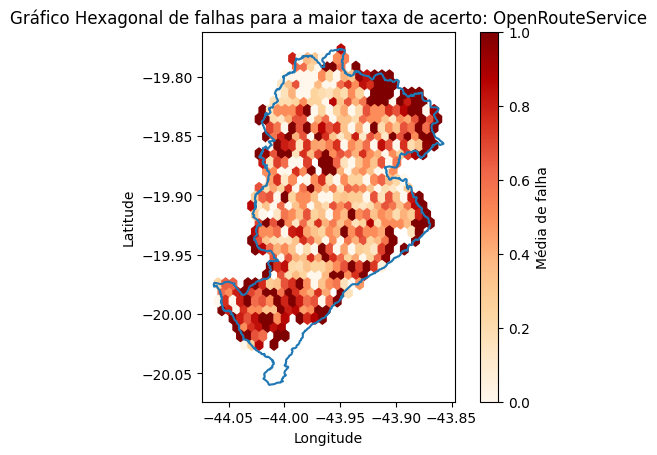
\includegraphics[width=\textwidth]{Figuras/expFalhasORSmaior.png}
%     \caption{Maior Taxa de Acerto}
%     \label{fig:falhasorsBHexpMaior}
%   \end{subfigure}
%   \hfill
%   \begin{subfigure}[b]{0.45\textwidth}
%     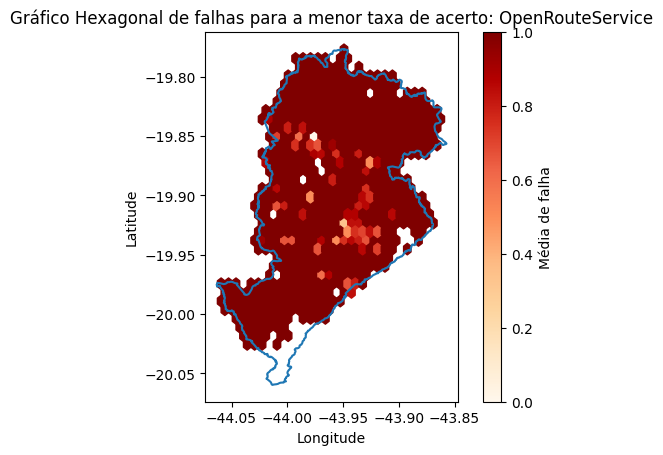
\includegraphics[width=\textwidth]{Figuras/expFalhasORSmenor.png}
%     \caption{Menor Taxa de Acerto}
%     \label{fig:falhasorsBHexpMenor}
%   \end{subfigure}
  
%   \caption{Gráficos de falhas para a maior e menor taxas de acerto dos experimentos para os dados de Belo Horizonte: Open Route Service}
%   \label{fig:falhas-exp-ors-bh}
% \end{figure}

% COLOCAR FALHAS ORS SP